\documentclass[11pt]{article}
% Shared preamble of the Korean reading editions of manuscripts A and B (XeLaTeX).
% Each main.tex loads it with % Shared preamble of the Korean reading editions of manuscripts A and B (XeLaTeX).
% Each main.tex loads it with % Shared preamble of the Korean reading editions of manuscripts A and B (XeLaTeX).
% Each main.tex loads it with \input{../common/preamble} after \documentclass[11pt]{article}.

\usepackage[a4paper,top=24mm,bottom=26mm,left=25mm,right=25mm,headheight=14pt]{geometry}

% Fonts: Latin in Times/Arial; Hangul in KoPubWorld (with a real bold) where installed,
% then Noto CJK KR, then the Batang and Malgun Gothic that ship with Windows.
\usepackage{fontspec}
\IfFontExistsTF{Times New Roman}{\setmainfont{Times New Roman}}{\setmainfont{TeX Gyre Termes}}
\IfFontExistsTF{Arial}{\setsansfont{Arial}[Scale=0.95]}{\setsansfont{TeX Gyre Heros}[Scale=0.95]}
\IfFontExistsTF{Consolas}{\setmonofont{Consolas}[Scale=0.9]}{}
\usepackage{kotex}
\IfFontExistsTF{KoPubWorldBatang Medium}{%
  \setmainhangulfont{KoPubWorldBatang Medium}[BoldFont={KoPubWorldBatang Bold},AutoFakeSlant=0.15]%
}{\IfFontExistsTF{Noto Serif CJK KR}{%
  \setmainhangulfont{Noto Serif CJK KR}[AutoFakeSlant=0.15]%
}{\setmainhangulfont{Batang}[AutoFakeSlant=0.15]}}
\IfFontExistsTF{KoPubWorldDotum Medium}{%
  \setsanshangulfont{KoPubWorldDotum Medium}[BoldFont={KoPubWorldDotum Bold},AutoFakeSlant=0.15]%
}{\IfFontExistsTF{Noto Sans CJK KR}{%
  \setsanshangulfont{Noto Sans CJK KR}[AutoFakeSlant=0.15]%
}{\setsanshangulfont{Malgun Gothic}[AutoFakeSlant=0.15]}}
\setmonohangulfont{Malgun Gothic}

\linespread{1.3}
\setlength{\parindent}{0pt}
\setlength{\parskip}{0.6em plus 0.2em minus 0.1em}
\setlength{\emergencystretch}{2em}
\raggedbottom

\usepackage{amsmath,amssymb}
\usepackage{array,booktabs,tabularx,multirow}
\usepackage{graphicx}
\usepackage[table]{xcolor}
\usepackage{tikz}
\usetikzlibrary{arrows.meta,positioning,calc}
\usepackage[most]{tcolorbox}
\usepackage{enumitem}
\setlist{itemsep=0.3em,topsep=0.2em,parsep=0.2em,leftmargin=1.7em}
\usepackage[font=small,labelfont={bf,sf},labelsep=period,justification=raggedright,
  singlelinecheck=false,skip=5pt]{caption}

\usepackage{titlesec}
\titleformat{\section}{\sffamily\Large\bfseries}{\thesection}{0.6em}{}
\titleformat{\subsection}{\sffamily\large\bfseries}{\thesubsection}{0.6em}{}
\titleformat{\subsubsection}{\sffamily\normalsize\bfseries}{\thesubsubsection}{0.6em}{}
\titleformat{\paragraph}[runin]{\sffamily\normalsize\bfseries}{}{0pt}{}
\titlespacing*{\section}{0pt}{1.4em}{0.5em}
\titlespacing*{\subsection}{0pt}{1.1em}{0.4em}
\titlespacing*{\subsubsection}{0pt}{0.9em}{0.3em}
\titlespacing*{\paragraph}{0pt}{0.6em}{0.6em}

\usepackage{fancyhdr}
\pagestyle{fancy}
\fancyhf{}
\renewcommand{\headrulewidth}{0.4pt}
\fancyhead[L]{\small\sffamily\ShortTitle}
\fancyhead[R]{\small\sffamily 쉬운 한국어 해설판}
\fancyfoot[C]{\small\thepage}
\newcommand{\ShortTitle}{}

\usepackage{longtable}
\usepackage{cite}
\PassOptionsToPackage{hyphens}{url}
\usepackage[hidelinks]{hyperref}
\urlstyle{same}

\renewcommand{\figurename}{그림}
\renewcommand{\tablename}{표}
\renewcommand{\refname}{참고문헌}
\renewcommand{\contentsname}{차례}

% Boxes. yoji: the gist of a section; puri: an explanation for the reader.
% Neither box is part of the English manuscript; the text outside the boxes is.
\newtcolorbox{yoji}{enhanced,breakable,colback=black!5,colframe=black!5,boxrule=0pt,arc=0pt,
  borderline west={2.5pt}{0pt}{black!50},left=9pt,right=8pt,top=5pt,bottom=5pt,
  before skip=0.5em,after skip=0.9em,fontupper=\small,
  before upper={\textsf{\textbf{요점}}\quad}}
\newtcolorbox{puri}[1][쉽게 풀면]{enhanced,breakable,colback=blue!3,colframe=blue!35!black!45,
  boxrule=0.5pt,arc=1.5pt,left=8pt,right=8pt,top=4pt,bottom=5pt,before skip=0.7em,after skip=0.9em,
  fontupper=\small,title={#1},fonttitle=\sffamily\bfseries\small,coltitle=black!85,
  colbacktitle=blue!9,toptitle=1pt,bottomtitle=1pt}

% Title block: \KoTitle{Korean title}{English title}{authors}{venue and source}
\newcommand{\KoTitle}[4]{%
  \thispagestyle{plain}%
  {\raggedright
  {\sffamily\bfseries\LARGE #1\par}\vspace{0.7em}
  {\large #2\par}\vspace{0.9em}
  {\small #3\par}\vspace{0.3em}
  {\small\color{black!70}#4\par}}
  \vspace{0.6em}\hrule\vspace{0.4em}}

% Numbers written only to illustrate (check_numbers.py skips what this wraps).
\newcommand{\ill}[1]{#1}
\newcommand{\dt}{\Delta\tau}
\newcommand{\Tobs}{T_{\mathrm{obs}}}
% A table cell that wraps.
\newcolumntype{L}[1]{>{\raggedright\arraybackslash}p{#1}}
\newcolumntype{Y}{>{\raggedright\arraybackslash}X}
 after \documentclass[11pt]{article}.

\usepackage[a4paper,top=24mm,bottom=26mm,left=25mm,right=25mm,headheight=14pt]{geometry}

% Fonts: Latin in Times/Arial; Hangul in KoPubWorld (with a real bold) where installed,
% then Noto CJK KR, then the Batang and Malgun Gothic that ship with Windows.
\usepackage{fontspec}
\IfFontExistsTF{Times New Roman}{\setmainfont{Times New Roman}}{\setmainfont{TeX Gyre Termes}}
\IfFontExistsTF{Arial}{\setsansfont{Arial}[Scale=0.95]}{\setsansfont{TeX Gyre Heros}[Scale=0.95]}
\IfFontExistsTF{Consolas}{\setmonofont{Consolas}[Scale=0.9]}{}
\usepackage{kotex}
\IfFontExistsTF{KoPubWorldBatang Medium}{%
  \setmainhangulfont{KoPubWorldBatang Medium}[BoldFont={KoPubWorldBatang Bold},AutoFakeSlant=0.15]%
}{\IfFontExistsTF{Noto Serif CJK KR}{%
  \setmainhangulfont{Noto Serif CJK KR}[AutoFakeSlant=0.15]%
}{\setmainhangulfont{Batang}[AutoFakeSlant=0.15]}}
\IfFontExistsTF{KoPubWorldDotum Medium}{%
  \setsanshangulfont{KoPubWorldDotum Medium}[BoldFont={KoPubWorldDotum Bold},AutoFakeSlant=0.15]%
}{\IfFontExistsTF{Noto Sans CJK KR}{%
  \setsanshangulfont{Noto Sans CJK KR}[AutoFakeSlant=0.15]%
}{\setsanshangulfont{Malgun Gothic}[AutoFakeSlant=0.15]}}
\setmonohangulfont{Malgun Gothic}

\linespread{1.3}
\setlength{\parindent}{0pt}
\setlength{\parskip}{0.6em plus 0.2em minus 0.1em}
\setlength{\emergencystretch}{2em}
\raggedbottom

\usepackage{amsmath,amssymb}
\usepackage{array,booktabs,tabularx,multirow}
\usepackage{graphicx}
\usepackage[table]{xcolor}
\usepackage{tikz}
\usetikzlibrary{arrows.meta,positioning,calc}
\usepackage[most]{tcolorbox}
\usepackage{enumitem}
\setlist{itemsep=0.3em,topsep=0.2em,parsep=0.2em,leftmargin=1.7em}
\usepackage[font=small,labelfont={bf,sf},labelsep=period,justification=raggedright,
  singlelinecheck=false,skip=5pt]{caption}

\usepackage{titlesec}
\titleformat{\section}{\sffamily\Large\bfseries}{\thesection}{0.6em}{}
\titleformat{\subsection}{\sffamily\large\bfseries}{\thesubsection}{0.6em}{}
\titleformat{\subsubsection}{\sffamily\normalsize\bfseries}{\thesubsubsection}{0.6em}{}
\titleformat{\paragraph}[runin]{\sffamily\normalsize\bfseries}{}{0pt}{}
\titlespacing*{\section}{0pt}{1.4em}{0.5em}
\titlespacing*{\subsection}{0pt}{1.1em}{0.4em}
\titlespacing*{\subsubsection}{0pt}{0.9em}{0.3em}
\titlespacing*{\paragraph}{0pt}{0.6em}{0.6em}

\usepackage{fancyhdr}
\pagestyle{fancy}
\fancyhf{}
\renewcommand{\headrulewidth}{0.4pt}
\fancyhead[L]{\small\sffamily\ShortTitle}
\fancyhead[R]{\small\sffamily 쉬운 한국어 해설판}
\fancyfoot[C]{\small\thepage}
\newcommand{\ShortTitle}{}

\usepackage{longtable}
\usepackage{cite}
\PassOptionsToPackage{hyphens}{url}
\usepackage[hidelinks]{hyperref}
\urlstyle{same}

\renewcommand{\figurename}{그림}
\renewcommand{\tablename}{표}
\renewcommand{\refname}{참고문헌}
\renewcommand{\contentsname}{차례}

% Boxes. yoji: the gist of a section; puri: an explanation for the reader.
% Neither box is part of the English manuscript; the text outside the boxes is.
\newtcolorbox{yoji}{enhanced,breakable,colback=black!5,colframe=black!5,boxrule=0pt,arc=0pt,
  borderline west={2.5pt}{0pt}{black!50},left=9pt,right=8pt,top=5pt,bottom=5pt,
  before skip=0.5em,after skip=0.9em,fontupper=\small,
  before upper={\textsf{\textbf{요점}}\quad}}
\newtcolorbox{puri}[1][쉽게 풀면]{enhanced,breakable,colback=blue!3,colframe=blue!35!black!45,
  boxrule=0.5pt,arc=1.5pt,left=8pt,right=8pt,top=4pt,bottom=5pt,before skip=0.7em,after skip=0.9em,
  fontupper=\small,title={#1},fonttitle=\sffamily\bfseries\small,coltitle=black!85,
  colbacktitle=blue!9,toptitle=1pt,bottomtitle=1pt}

% Title block: \KoTitle{Korean title}{English title}{authors}{venue and source}
\newcommand{\KoTitle}[4]{%
  \thispagestyle{plain}%
  {\raggedright
  {\sffamily\bfseries\LARGE #1\par}\vspace{0.7em}
  {\large #2\par}\vspace{0.9em}
  {\small #3\par}\vspace{0.3em}
  {\small\color{black!70}#4\par}}
  \vspace{0.6em}\hrule\vspace{0.4em}}

% Numbers written only to illustrate (check_numbers.py skips what this wraps).
\newcommand{\ill}[1]{#1}
\newcommand{\dt}{\Delta\tau}
\newcommand{\Tobs}{T_{\mathrm{obs}}}
% A table cell that wraps.
\newcolumntype{L}[1]{>{\raggedright\arraybackslash}p{#1}}
\newcolumntype{Y}{>{\raggedright\arraybackslash}X}
 after \documentclass[11pt]{article}.

\usepackage[a4paper,top=24mm,bottom=26mm,left=25mm,right=25mm,headheight=14pt]{geometry}

% Fonts: Latin in Times/Arial; Hangul in KoPubWorld (with a real bold) where installed,
% then Noto CJK KR, then the Batang and Malgun Gothic that ship with Windows.
\usepackage{fontspec}
\IfFontExistsTF{Times New Roman}{\setmainfont{Times New Roman}}{\setmainfont{TeX Gyre Termes}}
\IfFontExistsTF{Arial}{\setsansfont{Arial}[Scale=0.95]}{\setsansfont{TeX Gyre Heros}[Scale=0.95]}
\IfFontExistsTF{Consolas}{\setmonofont{Consolas}[Scale=0.9]}{}
\usepackage{kotex}
\IfFontExistsTF{KoPubWorldBatang Medium}{%
  \setmainhangulfont{KoPubWorldBatang Medium}[BoldFont={KoPubWorldBatang Bold},AutoFakeSlant=0.15]%
}{\IfFontExistsTF{Noto Serif CJK KR}{%
  \setmainhangulfont{Noto Serif CJK KR}[AutoFakeSlant=0.15]%
}{\setmainhangulfont{Batang}[AutoFakeSlant=0.15]}}
\IfFontExistsTF{KoPubWorldDotum Medium}{%
  \setsanshangulfont{KoPubWorldDotum Medium}[BoldFont={KoPubWorldDotum Bold},AutoFakeSlant=0.15]%
}{\IfFontExistsTF{Noto Sans CJK KR}{%
  \setsanshangulfont{Noto Sans CJK KR}[AutoFakeSlant=0.15]%
}{\setsanshangulfont{Malgun Gothic}[AutoFakeSlant=0.15]}}
\setmonohangulfont{Malgun Gothic}

\linespread{1.3}
\setlength{\parindent}{0pt}
\setlength{\parskip}{0.6em plus 0.2em minus 0.1em}
\setlength{\emergencystretch}{2em}
\raggedbottom

\usepackage{amsmath,amssymb}
\usepackage{array,booktabs,tabularx,multirow}
\usepackage{graphicx}
\usepackage[table]{xcolor}
\usepackage{tikz}
\usetikzlibrary{arrows.meta,positioning,calc}
\usepackage[most]{tcolorbox}
\usepackage{enumitem}
\setlist{itemsep=0.3em,topsep=0.2em,parsep=0.2em,leftmargin=1.7em}
\usepackage[font=small,labelfont={bf,sf},labelsep=period,justification=raggedright,
  singlelinecheck=false,skip=5pt]{caption}

\usepackage{titlesec}
\titleformat{\section}{\sffamily\Large\bfseries}{\thesection}{0.6em}{}
\titleformat{\subsection}{\sffamily\large\bfseries}{\thesubsection}{0.6em}{}
\titleformat{\subsubsection}{\sffamily\normalsize\bfseries}{\thesubsubsection}{0.6em}{}
\titleformat{\paragraph}[runin]{\sffamily\normalsize\bfseries}{}{0pt}{}
\titlespacing*{\section}{0pt}{1.4em}{0.5em}
\titlespacing*{\subsection}{0pt}{1.1em}{0.4em}
\titlespacing*{\subsubsection}{0pt}{0.9em}{0.3em}
\titlespacing*{\paragraph}{0pt}{0.6em}{0.6em}

\usepackage{fancyhdr}
\pagestyle{fancy}
\fancyhf{}
\renewcommand{\headrulewidth}{0.4pt}
\fancyhead[L]{\small\sffamily\ShortTitle}
\fancyhead[R]{\small\sffamily 쉬운 한국어 해설판}
\fancyfoot[C]{\small\thepage}
\newcommand{\ShortTitle}{}

\usepackage{longtable}
\usepackage{cite}
\PassOptionsToPackage{hyphens}{url}
\usepackage[hidelinks]{hyperref}
\urlstyle{same}

\renewcommand{\figurename}{그림}
\renewcommand{\tablename}{표}
\renewcommand{\refname}{참고문헌}
\renewcommand{\contentsname}{차례}

% Boxes. yoji: the gist of a section; puri: an explanation for the reader.
% Neither box is part of the English manuscript; the text outside the boxes is.
\newtcolorbox{yoji}{enhanced,breakable,colback=black!5,colframe=black!5,boxrule=0pt,arc=0pt,
  borderline west={2.5pt}{0pt}{black!50},left=9pt,right=8pt,top=5pt,bottom=5pt,
  before skip=0.5em,after skip=0.9em,fontupper=\small,
  before upper={\textsf{\textbf{요점}}\quad}}
\newtcolorbox{puri}[1][쉽게 풀면]{enhanced,breakable,colback=blue!3,colframe=blue!35!black!45,
  boxrule=0.5pt,arc=1.5pt,left=8pt,right=8pt,top=4pt,bottom=5pt,before skip=0.7em,after skip=0.9em,
  fontupper=\small,title={#1},fonttitle=\sffamily\bfseries\small,coltitle=black!85,
  colbacktitle=blue!9,toptitle=1pt,bottomtitle=1pt}

% Title block: \KoTitle{Korean title}{English title}{authors}{venue and source}
\newcommand{\KoTitle}[4]{%
  \thispagestyle{plain}%
  {\raggedright
  {\sffamily\bfseries\LARGE #1\par}\vspace{0.7em}
  {\large #2\par}\vspace{0.9em}
  {\small #3\par}\vspace{0.3em}
  {\small\color{black!70}#4\par}}
  \vspace{0.6em}\hrule\vspace{0.4em}}

% Numbers written only to illustrate (check_numbers.py skips what this wraps).
\newcommand{\ill}[1]{#1}
\newcommand{\dt}{\Delta\tau}
\newcommand{\Tobs}{T_{\mathrm{obs}}}
% A table cell that wraps.
\newcolumntype{L}[1]{>{\raggedright\arraybackslash}p{#1}}
\newcolumntype{Y}{>{\raggedright\arraybackslash}X}

\renewcommand{\ShortTitle}{원고 B · IEEE Access}

\newtheorem{proposition}{명제}
\newenvironment{proofko}{\par\noindent\textsf{\textbf{증명.}}\ }{\hfill$\square$\par}
% Colours of the two layers in Fig. 1 (as in the English figures/fig_layers_standalone.tex)
\definecolor{authc}{HTML}{EB6834}
\definecolor{payc}{HTML}{2A78D6}
\newcommand{\sha}[1]{\texttt{\footnotesize #1}}
% A centred table cell that wraps, and a coefficient with its interval on two lines.
\newcolumntype{C}[1]{>{\centering\arraybackslash}p{#1}}
\newcommand{\tc}[2]{#1\newline #2}

\begin{document}

\KoTitle{허락 층과 송금 층을 한 페이지랭크 걷기로 묶은 스마트 계약 평판\\[0.25em]\Large 이더리움 롤업에서 미리 정하고 커밋으로 잠근 기간 밖 시험}
{Coupling Authorization and Payment Layers in a PageRank Walk for Smart-Contract Reputation: A Pre-Specified, Commit-Gated Out-of-Window Test on an Ethereum Rollup}
{Taehong Kwon, Ernest Mnkandla, Donatien Koulla Moulla, David Sena Attipoe\\
School of Computing, University of South Africa}
{IEEE Access에 낼 원고 B(Research Article)의 쉬운 한국어 해설판 · 영문 원고: 원고 저장소 \texttt{07391e9}의 \texttt{manuscripts/B-ieee-access}}

\section*{이 글을 읽는 법}

\begin{itemize}
\item 영문 원고 B를 쉬운 한국어로 풀어 쓴 글이에요. 절의 순서는 영문 원고와 같고, 영문 원고의 I–X절이 여기서는 1–10절, 부록 A는 그대로 부록 A예요. 하지만 문장을 하나하나 옮긴 번역은 아니에요.
\item 회색 \textsf{\textbf{요점}} 상자는 그 절의 핵심이고, 파란 상자는 낯선 개념과 표 읽는 법을 풀어 줘요. 두 상자는 영문 원고에 없어요. 상자 밖 본문이 영문 원고의 내용이에요.
\item 수와 구간은 모두 영문 원고와 같아요. “+0.170 [0.149, 0.189]”는 두 점수의 타우 차이 +0.170과 그 95\% 신뢰구간이에요. 이 원고의 구간은 판정 규칙의 것이든 명목상 결과의 것이든 모두 짝지은 부트스트랩의 95\% 구간이에요. 판정은 그 구간의 한쪽 끝으로 내려요. 우월성은 아래 끝이 0보다 위인지, 비열등성은 아래 끝이 허용 폭 −0.01보다 위인지, “더 나쁘지 않음”은 위 끝이 0 이상인지를 봐요.
\end{itemize}

{\small\setcounter{tocdepth}{1}\tableofcontents}

%======================================================================
\section*{한눈에 보기: 초록}
\addcontentsline{toc}{section}{한눈에 보기: 초록}

\paragraph{무엇을 묻나요?}
블록체인 평판 점수는 보통 토큰 송금으로 주소의 순위를 매겨요. 그런데 같은 주소들은 허락으로도 이어져 있어요. 허락은 주인이 스펜더에게 자기 토큰을 옮겨도 된다고 허락한 기록이에요. 이 원고는 송금과 허락을 한 네트워크의 두 층으로 보고 물어요. 모든 점에서 두 층을 섞어 걷는 무작위 걷기가, 한 층만 걷는 것보다 스마트 계약의 순위를 더 잘 매길까요? 자료는 아비트럼 원(Arbitrum One)이에요.

\paragraph{무엇을 비교했나요?}
\begin{itemize}
\item C-PR(결합 페이지랭크): 점마다 허락 층과 송금 층의 행을 섞는 비율 $\lambda$로 섞어 걸어요. 주 설정은 $\lambda=0.5$예요.
\item 허락 걷기($\lambda=1$)와 송금 걷기($\lambda=0$): C-PR의 두 끝점으로, 한 층만 걸어요. 두 판정 규칙은 C-PR을 이 둘과 견줘요.
\item S-PR: 송금 층을 걷되 허락 걷기의 점수로 다시 출발하는 빼 보기 실험이에요.
\item 짝 원고의 기준 점수: 엔도스랭크, AWP, 그리고 원시 차수 두 가지(받은 허락 수, 송금 입차수).
\end{itemize}
판정 규칙 두 개는, 이 연구가 그 규칙으로 판정할 평가 로그를 추출하기 전에 저자들의 공개 저장소에 커밋했어요. 두 번째 규칙은 2026년 7–9월 창의 로그를 질의하기 8초 전에 커밋했어요. 그 질의를 돌린 코드는 커밋된 파일을 확인한 뒤에야 돌아요.

주 분석은 서로 다른 주인 셋 이상에게 허락을 받은 계약 6,483개를, 각 동결 직전 12개월 동안 다섯 토큰의 달러 금액으로 점수 매겨요. 이 세 가지(달러 금액, 다섯 토큰, 12개월 점수 기간)는 계획의 결과를 안 뒤에 정했으므로, 주 분석은 재분석이에요.

\paragraph{무엇을 찾았나요?}
\begin{enumerate}
\item \textbf{두 규칙 모두 만족하지 못했어요.}
\item \textbf{나중의 허락은 더 잘 맞혔어요.} 결합 걷기는 나중에 허락을 얻은 계약을 송금 걷기보다 잘 줄 세웠어요(순위 상관 차이 0.170, 95\% 구간 [0.149, 0.189]).
\item \textbf{나중의 송금은 허용 폭보다 더 못 맞혔어요.} 나중에 송금해 온 주소는 송금 걷기만큼 잘 줄 세우지 못했고, 그 차이가 허용 폭 0.01을 넘었어요(−0.025, 구간 [−0.038, −0.015]).
\item \textbf{트레이더에서는 같았지만 정밀하지 못했어요.} 계약 트레이더가 청산 없이 거래한 비율에서는, 주 분석에서 송금 걷기와 같았지만 구간이 넓어 허용 폭 안에 머물지 못했어요.
\item \textbf{원시 차수보다 못했어요.} 수정 분석에서 라벨을 안 뒤에 계산한 대비로는, 결합 걷기가 두 창 모두에서 나중의 허락을 허락한 주인 수(원시 차수)만큼 잘 줄 세우지 못했어요(두 번째 창 −0.065, 구간 [−0.077, −0.054]).
\item \textbf{원래 단위로 미리 정한 분석도 같은 판정에 이르렀어요.}
\item \textbf{적은 주소로 부풀릴 수 있어요.} 사후 모형에서, 짜고 움직이는 주소 26개면 목표 계약의 허락 점수를 코호트의 10분의 9보다 위로 올릴 수 있어요.
\end{enumerate}

\paragraph{무엇을 조심해야 하나요?}
수정 분석(달러 금액, 다섯 토큰, 동결 직전 12개월 점수 기간)은 등록 분석의 결과를 안 뒤에 정했으므로, 그 판정은 등록한 시험이 아니라 재분석이에요. 등록이 추출보다 먼저였다는 것은 커밋 시각과 작업 시각에 기대고, 제3자의 시간 도장에 기대지 않아요. 원시 차수와 기준 걷기와의 대비, 그리고 농장 모형은 라벨을 안 뒤에 계산했고 어느 규칙에도 들어가지 않아요. 트레이더는 70개뿐이에요.

\begin{puri}[한 문장으로 줄이면]
허락 층을 송금 걷기에 섞으면 나중의 새 허락은 더 잘 맞히지만 나중의 새 송금자는 송금 걷기보다 못 맞혀서(규칙 B에서는 허용 폭보다 더), 미리 정한 두 규칙을 모두 통과하지 못했어요. 그리고 수정 분석에서 라벨을 안 뒤에 계산한 대비로는, 결합 걷기가 두 창 모두에서 원시 차수(화살표를 그냥 센 수)만큼 잘 줄 세우지 못했어요.
\end{puri}

%======================================================================
\section*{먼저 알아 둘 말}
\addcontentsline{toc}{section}{먼저 알아 둘 말}

{\small
\renewcommand{\arraystretch}{1.25}
\begin{longtable}{@{}L{3.6cm}L{\dimexpr\linewidth-3.6cm-2\tabcolsep\relax}@{}}
\toprule
말 & 뜻 \\
\midrule
\endfirsthead
\toprule
말 & 뜻 \\
\midrule
\endhead
\bottomrule
\endlastfoot
스마트 계약(계약) & 블록체인 위에서 저절로 실행되는 프로그램이에요. 이 원고가 점수를 매기는 대상은 처음부터 끝까지 계약이에요. \\
외부 소유 계정(EOA) & 개인 키로 움직이는 계정이에요. 그래프에는 주인, 보낸 쪽, 받는 쪽으로만 나오고 점수를 받지 않아요. \\
허락(allowance) & 토큰 주인이 스펜더에게 “내 토큰을 이만큼까지 꺼내 써도 된다”고 허락한 기록이에요. \texttt{approve}를 부르거나 \texttt{permit}에 서명해서 정해요. 돈을 옮기지는 않아요. \\
주인, 스펜더 & 허락을 해 주는 쪽과, 허락을 받아 대신 쓰는 쪽이에요. \\
송금(transfer) & 토큰이 한 주소에서 다른 주소로 옮겨진 기록이에요. \\
허락 층, 송금 층 & 같은 주소들 위에 놓인 두 그래프예요. 허락 층의 화살표는 주인 → 스펜더(양수인 마지막 허락), 송금 층의 화살표는 보낸 쪽 → 받는 쪽이에요. 영문 원고는 두 층을 authorization layer, payment layer라고 불러요. \\
원시 차수 & 화살표를 그냥 센 수예요. 받은 허락 수(그 계약에 양수의 마지막 허락을 둔 서로 다른 주인 수)와 송금 입차수(그 계약에 송금한 서로 다른 주소 수)를 써요. \\
페이지랭크 & 화살표를 따라 무작위로 걷다가 가끔 다시 출발할 때, 아주 오래 걸으면 각 점에 머무는 비율이에요. 화살표를 따라갈 확률(감쇠 계수)은 $d=0.85$예요. \\
매달린 점 & 나가는 화살표가 없는 점이에요. 걷는 사람이 여기에 오면 다시 출발 분포를 따라 뛰어요. \\
C-PR(결합 페이지랭크) & 점마다 허락 층의 행과 송금 층의 행을 섞는 비율 $\lambda$로 섞어 걷는 페이지랭크예요. 주 설정은 $\lambda=0.5$예요. \\
허락 걷기, 송금 걷기 & C-PR의 두 끝점이에요. $\lambda=1$이면 허락 층만, $\lambda=0$이면 송금 층만 걸어요. 두 규칙은 C-PR을 이 둘과 견줘요. \\
S-PR(보증 씨앗 페이지랭크) & 송금 층을 걷되, 다시 출발할 곳을 허락 걷기의 점수에 비례해 고르는 빼 보기 실험이에요. \\
엔도스랭크, AWP & 짝 원고의 기준 걷기예요. 엔도스랭크는 허락 층을, AWP는 송금 층을 상한이 있는 무게로 걸어요. AWP는 최근에 활발히 송금한 주소에서 더 자주 다시 출발해요. \\
동결, 점수 기간 & 점수를 고정하는 시점이 동결이에요. 수정 분석은 동결 직전 12개월(점수 기간)의 사건으로만 점수를 만들어요. \\
라벨, W0, W1 & 동결 뒤 석 달 동안 생긴 일로 센 값이 라벨이에요. W0은 2026년 3월 31일에 동결하고 4–6월을, W1은 2026년 6월 30일에 동결하고 7–9월을 라벨 기간으로 써요. \\
새 허락 쌍, 새 송금자 & 라벨 기간에 그 계약에 새로 양수의 허락을 준 주인과, 새로 송금해 온 주소예요. \\
청산 없이 닫은 비율 & GMX V2에서 거래하는 계약이 라벨 기간에 닫은 포지션 가운데 강제 청산이 아니었던 몫이에요. \\
켄달의 타우($\tau_b$) & 두 줄 세우기가 얼마나 같은 순서인지 나타내는 수예요. 1이면 순서가 완전히 같고, 0이면 순서의 경향이 없고, −1이면 정반대예요. 동점을 바로잡은 꼴($\tau_b$)을 써요. \\
$\Delta\tau$ & 두 점수의 타우 차이, $\tau_a-\tau_b$예요. 양수면 $a$가 라벨을 더 잘 줄 세운 거예요. \\
짝지은 부트스트랩, 95\% 구간 & 계약을 되돌려 넣으며 다시 뽑아 같은 계산을 되풀이하고, 결과의 가운데 95\%가 놓인 범위를 구간으로 써요. 한 라벨의 모든 점수가 같은 다시 뽑기를 쓰므로, 두 점수의 차이는 짝지은 차이예요. \\
규칙 A, 규칙 B & 미리 정한 판정 규칙 두 개예요. 규칙 A는 분석 계획에 있어요. 주 부분은 W0으로, 부 부분은 같은 기간의 점검으로 판정해요. 규칙 B는 W1 등록 문서에 있고 W1로 판정해요. \\
우월성, 비열등성, 더 나쁘지 않음 & 차이의 구간이 통째로 0보다 위면 우월성, 구간의 아래 끝이 $-\delta$보다 위면 비열등성, 구간이 0을 포함하거나 0보다 위면 “더 나쁘지 않음”이에요. \\
허용 폭 $\delta$ & 규칙 B의 비열등성 기준 0.01이에요. 이만큼까지 뒤지는 것은 봐줘요. W0 스펜더 대비의 정밀도에서 정한 값이지, 실제로 중요하다고 판단한 차이가 아니에요. \\
명목상의 판정 & 판정 규칙에 들어가지 않고, 보정하지 않은 95\% 구간으로 하나씩 따로 내린 판정이에요. \\
등록 분석 & 분석 계획과 W1 등록 문서에 정한 그대로 한 분석이에요. 금액은 원래 단위, 토큰은 모든 ERC-20, 점수는 2023년 10월 1일부터의 모든 사건으로 만들었어요. 두 규칙은 이 분석을 위해 정한 시험이에요. \\
수정 분석, 재분석 & 등록 분석의 결과를 안 뒤에 정한 분석으로, 금액은 달러, 토큰은 다섯 개, 점수는 동결 직전 12개월의 사건으로 만들어요. 원고의 주 분석이고, 등록한 규칙을 여기에 적용한 것은 재분석이라고 불러요. \\
커밋으로 잠근 추출 & 등록 파일이 로컬 수정 없이 커밋되어 있어야만 W1 로그를 추출하는 스크립트가 도는 방식이에요. 스크립트는 그 파일들의 SHA-256 해시를 매니페스트에 적어요. \\
시빌 공격, 농장 & 가짜 주소를 많이 만들어 점수를 속이는 공격과, 공격자가 만든 주소 무리예요. \\
\end{longtable}}
\addtocounter{table}{-1}% the glossary is not a numbered table

%======================================================================
\section{들어가며}
\label{sec:intro}

\begin{yoji}
블록체인 평판 점수는 보통 송금 그래프를 걸어요. 그런데 같은 주소들은 허락으로도 이어져 있어요. 이 원고는 두 관계를 한 걷기로 섞으면 계약의 순위를 더 잘 매기는지를, 미리 정해 커밋한 두 규칙으로 시험해요. 두 규칙은 모두 실패했어요.
\end{yoji}

\subsection{디파이는 주소로만 아는 상대와 거래해요}

디파이(DeFi, 탈중앙 금융)의 대출과 마진 거래 프로토콜은 주소로만 아는 상대와 연동을 다뤄요~\cite{schar2021defi}. 그래서 신용 기록 대신 과담보(빌리는 돈보다 담보를 더 맡기기)와 자동 청산에 기대요~\cite{gudgeon2020crisis,werner2022sok}. 한 갈래의 연구는 빠진 정보를 공개 장부에서 얼마쯤 되찾으려 해요. 그 대부분은 토큰 송금 그래프 위에서 주소의 순위를 매겨요.
\begin{itemize}
\item Do와 Do는 이더리움 거래 위의 페이지랭크와 호지랭크(HodgeRank)를 사회적 신용의 척도로 읽어요~\cite{do2023hodgerank}.
\item Do, Do, Nguyen의 AWP(적응형 가중 페이지랭크)는 송금마다 금액과 나이로 무게를 달고, 최근에 활발히 송금한 주소에서 걷기를 다시 출발시켜요~\cite{do2023awp}.
\item RiskProp은 거래 네트워크를 따라 계정의 위험을 퍼뜨려요~\cite{lin2025riskprop}.
\end{itemize}
블록체인 평판 시스템을 살핀 조사도 같은 의존, 곧 송금량이나 명시적 평가에 기대는 모습을 찾아요~\cite{bellini2020trust}. 이런 점수는 누구나 공개 사건으로 다시 계산할 수 있어요. 그래서 탈중앙 신용 평가가 속을 알 수 없는 블랙박스가 된다는 걱정에 얼마쯤 답해요~\cite{packin2024credit}.

\subsection{장부는 두 번째 관계도 기록해요}

송금은 지급을 기록해요. 그런데 장부는 같은 주소들 사이의 두 번째 관계도 기록해요. ERC-20(Ethereum Request for Comments 20) 토큰 규칙에서 주인은 \texttt{approve}를 불러, 스펜더가 자기 토큰을 정한 양까지 꺼내 쓰게 해요. EIP 2612(Ethereum Improvement Proposal)의 \texttt{permit} 함수는 블록체인 밖의 서명으로 같은 허락을 정해요~\cite{vogelsteller2015erc20,lundfall2020permit}.

허락은 돈을 옮기지 않아요. 스펜더가 나중에 쓸 수 있는 능력을 줄 뿐이고, 주인은 그 허락을 올리거나 내리거나 거둘 수 있어요. 그리고 많은 허락이 무제한이에요~\cite{wang2022unlimited}. 허락은 주로 사용자 계정에서 그 계정이 쓰는 라우터, 금고(vault), 거래 계약 쪽을 가리켜요. 그래서 허락은 스마트 계약의 순위를 매기는 데 자연스러운 신호예요. 이렇게 지급(송금)과 허락은 한 주소 집합 위의 두 층을 이뤄요. 다층 순위 매기기가 다루는 바로 그 상황이에요~\cite{halu2013multiplex,dedomenico2015ranking}.

\subsection{이 원고가 묻는 것}

이 원고는 이렇게 물어요. 두 층을 함께 걷는 무작위 걷기 하나가, 한 층만 걷는 것보다 계약의 순위를 더 잘 매길까요? 특히 송금 걷기에 허락 화살표를 더하면 나아질까요? 이를 위해 두 가지를 정의해요.
\begin{itemize}
\item \textbf{C-PR(결합 페이지랭크):} 점마다 두 층의 이동 행을 섞어요. 허락 층에는 고정된 무게 $\lambda$를 줘요.
\item \textbf{S-PR(보증 씨앗 페이지랭크):} 빼 보기 실험이에요. 송금 층을 걷되, 다시 출발할 곳을 허락 걷기에서 뽑아요. 트러스트랭크(TrustRank)가 미리 검증한 씨앗 집합에서 다시 출발하는 것과 같은 생각이에요~\cite{gyongyi2004trustrank}.
\end{itemize}
C-PR 가족의 끝점인 $\lambda=1$과 $\lambda=0$은 한 층만 걸어요. 이 둘이 두 판정 규칙의 비교 대상이에요. 점수를 받는 것은 처음부터 끝까지 스마트 계약이에요. 외부 소유 계정은 주인, 보낸 쪽, 받는 쪽으로 그래프에 들어가지만, 점수를 받지 않아요.

\subsection{시간을 앞으로 보는 평가}

평가는 시간을 앞으로 봐요. 어느 날짜에 점수를 동결하고, 그 뒤에 일어나는 결과와의 켄달 순위 상관으로 판단해요~\cite{kendall1938rank}. 결과는 세 가지예요.
\begin{itemize}
\item 그 계약에 새로 허락하는 주인.
\item 그 계약에 새로 송금하는 주소.
\item GMX V2 무기한 선물 거래소~\cite{gmxnddocs}에서 거래하는 계약이라면, 포지션 닫기 가운데 강제 청산을 피한 몫.
\end{itemize}
앞의 둘은 층을 이루는 것과 같은 종류의 화살표가 새로 생기는 것이에요. 셋째는 어느 층으로도 만들지 않았고, 이 자료에서 상대방 위험에 가장 가까운 결과예요~\cite{perez2021liquidations}.

\subsection{미리 정한 두 규칙과 그 결과}

판정 규칙 두 개를, 이 연구가 그 규칙으로 판정할 자료를 추출하기 전에 정했어요.
\begin{itemize}
\item \textbf{분석 계획:} 규칙 A와 모든 점수를 정했어요. 관측 기간을 복사한 BigQuery 작업이 만들어지기 10초 전에 저자들의 공개 저장소에 커밋했어요.
\item \textbf{두 번째 창의 등록:} 비열등성 허용 폭이 있는 규칙 B를 정했어요. 2026년 7–9월 로그를 복사한 작업보다 8초 먼저 커밋했어요. 그 작업을 돌리는 스크립트는 등록 파일이 로컬 수정 없이 커밋되어 있지 않으면 시작하지 않아요. 시작하면 그 파일들의 SHA-256 해시를 매니페스트에 적어요.
\end{itemize}
이 원고는 이런 방식을 “커밋으로 잠근(commit-gated)” 방식이라고 불러요. 두 커밋이 추출보다 먼저였다는 것은 커밋 시각과 작업 시각에 기대요. 제3자의 시간 도장에 기대는 것은 아니에요(\ref{sec:gate}절).

두 규칙은 모두 실패했어요. 이 결과를 안 뒤, 저자들은 계획이 금액에 무게를 다는 방식에서 결함 세 가지를 찾았어요. 그리고 이 원고가 먼저 보고하는 분석을 다음 세 가지로 정의했어요.
\begin{itemize}
\item 가격이 믿을 만한 다섯 토큰의 달러 금액.
\item 무제한 허락에 두는 상한.
\item 동결 직전 12개월의 사건으로 만든 점수.
\end{itemize}
계획대로라면 금액이 아무 효과가 없거나, 무제한 허락이 행을 다 차지했어요. 그래서 이 원고는 이 수정 분석을 앞에 둬요. 하지만 그 정의(달러 금액, 다섯 토큰, 12개월 점수 기간)가 결과 뒤에 나왔으므로, 그 판정은 같은 규칙에 따른 재분석이에요. 미리 정한 분석은 같은 판정에 이르렀고, 결과의 모든 표와 그림에서 수정 분석 옆에 함께 보고해요.

\subsection{기여}

\begin{enumerate}
\item \textbf{계약 평판의 두 층 모형.} 결합 걷기, 씨앗을 쓰는 빼 보기 실험, 분석적 관찰 두 가지를 내놓아요.
  \begin{itemize}
  \item $\lambda$가 0과 1 사이에 있을 때, 무게는 두 층 모두에 나가는 화살표가 있는 점을 통해서만 작용해요.
  \item 스펜더를 허락한 주인들이 스스로는 허락을 받지 않는 그래프에서, 허락 걷기는 주인 쪽에서 정규화한 받은 무게로 줄어들어요.
  \end{itemize}
\item \textbf{장부 자료 위의 순위 실험을 위한, 미리 정하고 커밋으로 잠근 절차.} 약속마다 날짜를 매기는 기록(\ref{sec:protocol}절)과 그 기록의 한계를 함께 내놓아요. 커밋 시각은 커밋한 사람의 시계가 정하고, 제3자의 시간 도장이 그 시각을 붙잡아 두지 않아요.
\item \textbf{아비트럼 원에서의 부정적 결과.} C-PR은 수정 분석에서도, 미리 정한 분석에서도 어느 규칙도 만족하지 못했어요.
  \begin{itemize}
  \item 나중의 허락에서 송금 걷기보다 나은 점은, 규칙을 정한 뒤 이 연구가 추출한 창에서도 유지됐어요.
  \item 하지만 나중의 송금자에서는 등록한 허용 폭보다 더 크게 뒤졌고, AWP에는 그보다 더 크게 뒤졌어요.
  \item 트레이더 결과에서는 허용 폭 안에 머물지 못했어요.
  \item 라벨을 안 뒤 계산한 짝지은 대비에서, C-PR은 수정 분석의 두 창 모두에서 나중의 허락은 허락한 주인 수만큼, 나중의 송금자는 서로 다른 송금자 수만큼 잘 줄 세우지 못했어요.
  \end{itemize}
\item \textbf{알려진 링크 농장 결과를 균등 재시작 아래의 허락 층에 맞춰 잰 사후 보정.} 수정 분석의 엔도스랭크 그래프에서, 닫힌 농장은 감쇠 계수 0.85에서 자기 인구 몫의 3.23배를 모아요. 농장 주소 26개, 약 2,292개, 약 47,073개짜리 별 모양은 목표를 코호트 엔도스랭크 점수의 90번째 백분위, 99번째 백분위, 꼭대기 위로 올려요. 등록 분석의 그래프에서는 이 수가 2.96, 13, 1,253, 약 1,080,271이에요.
\end{enumerate}

\subsection{짝 원고와 나눠 맡은 것}

짝 원고~\cite{kwon2026companion}는 두 화살표 종류를 따로따로의 점수로 견주고, 각 점수를 그 원시 차수와 견줘요. 그리고 어느 화살표로도 만들지 않은 트레이더 결과를 세 규칙(R1–R3)으로 다뤄요. 이 세 규칙은 규칙 B와 같은 커밋에 등록했어요.
\begin{itemize}
\item \textbf{두 원고가 함께 보고하는 것:} 같은 자료, 스펜더 홀드아웃에서 원시 차수·엔도스랭크·AWP의 계수와 차수 대비, 허락 걷기의 닫힌 식, 풀이 실행 시간.
\item \textbf{짝 원고에만 있는 것:} 트레이더 결과에서 허락 쪽과 송금 쪽을 견준 비교(그 연구의 규칙 R1–R3).
\item \textbf{이 원고가 같은 트레이더 코호트에서 보고하는 것:} 규칙 B와 그 등록 민감도 분석이 이름 붙인 C-PR의 대비, 그리고 라벨을 안 뒤에 계산한 C-PR과 받은 허락 수의 대비 하나.
\end{itemize}
두 원고 모두 수정 분석을 먼저 보고하고 등록 분석의 값을 옆에 둬요. 그리고 두 원고는 두 분석 모두에서 서로 같은 값을 보고해요. 이 원고가 다루는 것은 결합 연산자, 미리 정한 두 규칙과 그 기록, 그리고 허락 층을 얼마나 조작할 수 있는지예요.

글의 차례는 이래요. \ref{sec:related}절은 관련 연구, \ref{sec:model}절은 모형, \ref{sec:protocol}절은 규칙과 그 기록, \ref{sec:data}절은 자료와 측정, \ref{sec:results}절은 결과, \ref{sec:sybil}절은 농장 공격의 보정, \ref{sec:threats}절은 타당성을 위협하는 것, \ref{sec:implications}절은 대출·마진 프로토콜에 주는 시사점, \ref{sec:conclusion}절은 결론이에요. 부록~\ref{app:explore}에는 탐색적 점검을 모았어요.

%======================================================================
\section{관련 연구}
\label{sec:related}

\begin{yoji}
장부 그래프의 평판 연구는 거의 송금만 걸었어요. 다층 순위 매기기와 개인화 페이지랭크는 두 층을 섞는 방법을 줘요. 차수는 링크 예측의 표준 기준선이라, 걷기는 그 걷기가 다듬는 원시 차수와 견줘 시험해야 해요. 페이지랭크 같은 대칭 함수는 시빌 공격에 안전할 수 없어요. 미리 정한 분석은, 분석하는 사람이 아직 결과를 살피지 않았다면 이미 있는 자료에도 쓸 수 있어요.
\end{yoji}

\subsection{장부 그래프로 만든 평판}

페이지랭크는 방향이 있는 그래프의 점들을, 감쇠 계수를 쓰는 무작위 걷기의 정상 분포로 줄 세워요~\cite{page1999pagerank,langville2006pagerank}. HITS(Hyperlink-Induced Topic Search)는 허브와 권위를 나누고~\cite{kleinberg1999hits}, 아이겐트러스트(EigenTrust)는 지역 신뢰 값을 정규화해서 파일 공유 네트워크의 참여자가 자기 위치를 부풀리지 못하게 해요~\cite{kamvar2003eigentrust}.

공개 장부에서는 이런 생각을 거의 송금에만 적용했어요. 위에서 말한 방법들~\cite{do2023hodgerank,do2023awp} 말고도 이런 연구가 있어요. 거래 그래프의 네트워크 임베딩은 계정마다의 특징보다 피싱 계정을 더 잘 찾아요~\cite{wu2022phishers}. 암호화폐 거래의 지식 발견을 살핀 조사는 차수와 금액에 바탕을 둔 중심성을 흔한 주소 서술자로 꼽아요~\cite{liu2021knowledge}.

허락은 문헌에 두 가지 역할로 나와요. 한 주체의 주소들을 묶는 휴리스틱으로~\cite{victor2020clustering}, 그리고 무제한일 때의 보안 위험으로요~\cite{wang2022unlimited}. 휴먼 패스포트(Human Passport) 같은 도구는 무게를 단 자격 증명으로 주소의 주인을 점수 매길 뿐, 주소 사이 관계의 순위를 매기지는 않아요~\cite{humanpassportnddocs}. 짝 연구~\cite{kwon2026companion}는 마지막 허락을 순위 매기기의 화살표로 써요. 이 원고는 그 화살표를 송금 화살표와 한 걷기 안에서 묶어요.

\subsection{다층 순위와 개인화 순위}

\begin{itemize}
\item 멀티플렉스 페이지랭크는 한 층에서 얻은 중심성이 다른 층의 걷기를 기울이게 해요~\cite{halu2013multiplex}.
\item De Domenico 외의 서로 이어진 다층 틀에서는, 걷는 사람이 층 안에서 움직이다가 층 사이를 갈아타요. 그리고 점들을 여러 층에 걸친 쓰임새(versatility)로 줄 세워요~\cite{dedomenico2015ranking}.
\item 주제별 페이지랭크와 개인화 페이지랭크는 이동 행렬 대신 순간 이동 벡터를 바꿔요~\cite{haveliwala2003topic,jeh2003personalized}.
\item 트러스트랭크는 손으로 확인한 씨앗 집합으로만 순간 이동하게 해서 웹 스팸을 아래로 내려요~\cite{gyongyi2004trustrank}.
\end{itemize}
C-PR은 앞의 다층 걷기들(멀티플렉스 페이지랭크, 서로 이어진 다층 틀)의 특수한 경우예요. 행의 합이 1인 행렬 두 개를 점마다 볼록 결합(가중 평균)하되, 무게는 전체에 하나뿐이고 층 사이에 점의 복사본을 두지 않아요. S-PR은 순간 이동 벡터를 바꾸는 방법들(주제별·개인화 페이지랭크, 트러스트랭크)에 속해요. 아래의 명제~\ref{prop:localize}은 페이지랭크에서 흔히 쓰는 1차 섭동 한계~\cite{langville2006pagerank}를 이 볼록 결합에 맞춘 것이에요. 같은 주소들 사이의 두 온체인 관계에서, 연구가 평가 자료를 추출하기 전에 정한 규칙으로 이런 구성을 시험한 연구를 저자들은 문헌에서 찾지 못했어요.

\subsection{차수 기준선}

선호적 연결에서는 새 링크가 이미 링크가 많은 점에 몰려요~\cite{barabasi1999scaling}. 자라는 네트워크를 잰 연구도 같은 경향을 보여요~\cite{newman2001clustering}. 그래서 차수에 바탕을 둔 점수는 링크 예측의 표준 기준선이고~\cite{libennowell2007link}, 이더리움 거래 네트워크에서도 그래요~\cite{lin2022tracking}. 그리고 차수끼리의 상관이 약한 그래프에서는 페이지랭크가 평균적으로 들어오는 화살표 수에 비례해요~\cite{fortunato2008indegree}. 따라서 걷기가 정보를 더한다는 주장은, 그 걷기가 다듬는 원시 차수와 견줘 시험해야 해요. 이 원고는 모든 걷기를 그것과 견줘요.

\subsection{조작과 시빌 저항}

신원이 공짜인 곳에서는 한 행위자가 여럿으로 보일 수 있어요~\cite{douceur2002sybil}. Gy\"{o}ngyi와 Garcia-Molina는 목표의 페이지랭크를 가장 많이 올리는 링크 농장과 동맹을 끌어냈어요~\cite{gyongyi2005alliances}. Cheng과 Friedman은 페이지랭크를 포함해 어떤 대칭 평판 함수도 시빌 공격에 안전할 수 없다는 것을 보였어요. 반면 믿을 만한 출처에서 나가는 흐름이나 경로로 계산하는 비대칭 함수 가운데는 안전한 것도 있어요~\cite{cheng2005sybilproof}. \ref{sec:sybil}절은 이 결과를 허락 층에 적용해요. 새 결과를 끌어내지 않고, 수치로 보정할 뿐이에요.

장부에서는 자전 거래가 송금 활동을 부풀려요~\cite{victor2021washtrading,cong2023washtrading}. 사람 증명 방식은 시빌 저항과 개인정보 보호를 맞바꿔요~\cite{siddarth2020watchmen}. 그리고 탈중앙 시스템을 살핀 최근 검토는 자격 증명 파밍을 그런 관문의 남은 약점으로 꼽아요~\cite{bordeianu2026sybil}.

\subsection{미리 정한 분석}

사전 등록은 가설을 시험하는 분석과 가설을 만드는 분석을 나눠요. 분석하는 사람이 아직 결과를 살피지 않았다면, 이미 있는 자료에도 사전 등록을 쓸 수 있어요~\cite{nosek2018preregistration}. 관측된 장부 자료에서는 시험 창의 사건이 일어나는 순간부터 체인 위에 있어요. 그래서 연구가 줄 수 있는 가장 강한 현실적 보증은, 규칙을 정할 때 그 사건을 아직 추출하지 않았다는 것이에요. 구성 타당도 이론은 뒤에서 중요해지는 주의를 하나 더해요. 점수는 그것이 따라가도록 설계된 것의 점검과 맞아야 하므로, 그런 일치는 독립적인 증거가 아니에요~\cite{cronbach1955construct}.

%======================================================================
\section{모형}
\label{sec:model}

\begin{yoji}
같은 주소들 위에 허락 층과 송금 층을 놓고, 그 위에서 페이지랭크, C-PR, S-PR, 기준 점수를 정의해요. 명제 두 개가 섞는 비율 $\lambda$가 어디서 작용하는지, 그리고 깊이 1인 스펜더에서 허락 걷기가 무엇을 계산하는지 말해 줘요. C-PR은 두 층의 화살표를 모두 걸어서, 표~\ref{tab:bench}의 점수 가운데 푸는 시간이 가장 길었어요.
\end{yoji}

\subsection{한 주소 집합 위의 두 층}

$V=V_A\cup V_T$는 두 층 가운데 어느 하나에라도 있는 주소의 집합이에요(그림~\ref{fig:layers}). 영문 원고는 낱말을 이렇게 나눠 써요. 층과 그 화살표와 그 걷기에는 authorization(허락 층), 화살표를 만드는 사건에는 approval(허락하기), 허락한 금액에는 allowance(허락 금액)를 써요. 둘째 층도 층은 payment(송금 층), 그 사건은 transfer(송금)로 나눠요.

\paragraph{허락 화살표.}
기준 시점까지 주인 $u$가 스펜더 $v$에게 남긴 마지막 \texttt{Approval} 사건이 적어도 한 토큰에서 양수이면, 허락 화살표 $u\to v$가 있어요. 마지막 값이 0이면 그 쌍은 지워져요. 이것이 처리 과정이 실제로 재는 것이고, 지금 유효한 허락과는 세 가지가 달라요.
\begin{itemize}
\item 점수 기간이 시작되기 전에 정해지고 그 기간 안에 다시 나오지 않은 허락은 보이지 않아요.
\item \texttt{transferFrom}으로 일부를 꺼내 쓴 유한 허락도, 허락한 값을 그대로 가져요. 허락을 쓸 때 토큰이 \texttt{Approval} 사건을 꼭 남기지는 않기 때문이에요.
\item Uniswap의 Permit2 같은 허락 관리자에게 허락한 주인은, 그 관리자로 가는 화살표만 가져요.
\end{itemize}

\paragraph{송금 화살표.}
$u$가 $v$에게 양수 금액의 송금을 적어도 하나 보냈으면 송금 화살표 $u\to v$가 있어요. 이더(ETH)는 \texttt{Transfer} 로그 없이 움직이므로, 감싼 이더(WETH)로만 송금 층에 들어가요.

\paragraph{금액으로 단 무게.}
이 원고가 다루는 연산자는 두 층 모두에 금액으로 무게를 달아요.
\begin{equation}
\tilde w_A(u,v)=\sum_{\text{토큰}} g\bigl(a^{\star}(u,v,\text{토큰})\bigr),
\label{eq:layerA}
\end{equation}
\begin{equation}
\tilde w_T(u,v)=\sum_{e:\,u\to v} x_e\,\sigma(\Delta t_e).
\label{eq:layerT}
\end{equation}
\begin{itemize}
\item $a^{\star}$는 마지막 허락, $x_e$는 송금 $e$의 금액이에요.
\item $\sigma(\Delta t)=1/(1+\exp(k(\Delta t-t_0)))$는 나이 $\Delta t$(일)로 매기는 로지스틱 할인이에요. AWP가 쓰는 꼴이에요~\cite{do2023awp}. AWP 논문은 매개변수 값을 정하지 않아서, $k=0.01$과 $t_0=180$은 저자들이 고른 값이에요. 나이는 기준 시점에서 거꾸로 재요.
\item 허락 층은 할인하지 않아요.
\item 주 분석인 수정 분석(\ref{sec:revision}절)은 금액을 다섯 토큰의 달러 값으로 재고, 허락마다 상한을 둬요: $g(a)=\min(a,U)$, $U=19{,}000$달러. 계획은 원래 단위, 모든 ERC-20 토큰, $g(a)=a$로 정했어요.
\end{itemize}
$o_A(u)$와 $o_T(u)$는 각 층에서 나가는 무게의 합이에요. $P_A$와 $P_T$는 행마다 합이 1이 되게 나눈(행 정규화한) 행렬이고, 그 층에 나가는 화살표가 없는 점의 행은 0이에요.

\begin{figure}[!ht]
\centering
\begin{tikzpicture}[>=Stealth, font=\small,
  acc/.style={circle, draw=black!70, thick, minimum size=7mm, inner sep=0pt, fill=white},
  con/.style={rectangle, draw=black!80, thick, minimum size=6.8mm, inner sep=0pt, fill=black!12},
  auth/.style={->, thick, dashed, draw=authc},
  pay/.style={->, thick, draw=payc}]
  \node[acc] (u)  at (0,0)        {$u$};
  \node[acc] (w)  at (0,1.4)      {$w$};
  \node[acc] (x)  at (2.4,-1.4)   {$x$};
  \node[con] (r)  at (2.4,0.75)   {$R$};
  \node[con] (s)  at (4.8,-0.35)  {$S$};
  \node[acc, draw=black!40, text=black!60] (z) at (7.0,-0.35) {$z$};
  \draw[auth] (u) to[bend left=14] (r);
  \draw[pay]  (u) to[bend right=14] (r);
  \draw[auth] (u) to[bend right=10] (s);
  \draw[auth] (w) -- (r);
  \draw[auth] (x) -- (s);
  \draw[pay]  (r) -- (x);
  \draw[pay]  (s) -- (z);
  \draw[auth] (-0.4,2.75) -- (0.4,2.75) node[right, text=black] {허락(양수인 마지막 허락, 주인 $\to$ 스펜더)};
  \draw[pay]  (-0.4,2.3) -- (0.4,2.3) node[right, text=black] {송금(토큰 송금, 보낸 쪽 $\to$ 받는 쪽)};
  \node[con, minimum size=3.4mm] at (5.3,1.55) {};
  \node[right] at (5.5,1.55) {코호트 계약(점수를 받음)};
  \node[acc, minimum size=3.6mm] at (5.3,1.1) {};
  \node[right] at (5.5,1.1) {주인이나 상대방};
  \node[align=left, anchor=north west, inner sep=1pt] at (-0.45,-2.0)
    {$u\in B$: C-PR의 행 $=\lambda P_A(u,\cdot)+(1-\lambda)P_T(u,\cdot)$\\
     $w$, $x$: 나가는 화살표가 허락뿐이라 $\lambda>0$이면 $P_A$를 따라감\\
     $R$, $S$: 나가는 화살표가 송금뿐이라 $\lambda<1$이면 $P_T$를 따라감};
\end{tikzpicture}
\caption{같은 주소 집합 위의 두 층(개념도). 네모는 점수를 받는 코호트 계약이고, 동그라미는 사용자 계정 같은 주인과 상대방이에요. $z$는 코호트 계약이 송금했기 때문에만 나타나는 주소예요. 두 층 모두에 나가는 화살표가 있는 점은 $u$뿐이라, $0<\lambda<1$에서 $\lambda$에 따라 달라지는 행은 $u$의 행뿐이에요. $\lambda=1$이면 송금 화살표와 $z$가 빠지고, 계약 $R$과 $S$는 매달린 점이 돼요. $\lambda=0$이면 허락 화살표가 빠지고, $w$는 그래프를 떠나고 $x$는 매달린 점이 돼요. S-PR은 실선 화살표만 걷고, 뛸 때마다 허락 걷기의 점수에 비례해 다시 출발해요.}
\label{fig:layers}
\end{figure}

\subsection{다시 출발 분포가 있는 페이지랭크}

아래의 모든 점수는 다음 식의 고정점이에요.
\begin{equation}
\mathbf r^{(t+1)}=(1-d)\,\boldsymbol\pi+d\,P^{\top}\mathbf r^{(t)}+d\,\bigl(\mathbf 1_{\mathrm{dang}}^{\top}\mathbf r^{(t)}\bigr)\,\boldsymbol\pi.
\label{eq:pr}
\end{equation}
$P$는 이동 행렬, $\boldsymbol\pi$는 다시 출발 분포예요. $\mathbf 1_{\mathrm{dang}}$은 행이 모두 0인 점(매달린 점)을 가리키는 표시이고, 그 점의 몫은 $\boldsymbol\pi$를 따라 다시 나눠져요. $d=0.85$를 쓰고, 균등한 벡터에서 시작해서, $\ell_1$ 변화가 $10^{-8}$ 아래로 내려가거나 300번 반복하면 멈춰요.

\begin{puri}[식~\eqref{eq:pr}을 말로 읽으면]
걷는 사람은 한 걸음마다 확률 $d$로 지금 점의 화살표 하나를 따라가고(무게가 큰 화살표일수록 자주), 확률 $1-d$로 $\boldsymbol\pi$를 따라 아무 점으로나 뛰어요. 나가는 화살표가 없는 매달린 점에 도착하면 그 몫도 $\boldsymbol\pi$를 따라 다시 나눠져요. 이 걸음을 되풀이해서 더는 바뀌지 않게 된 값이 각 점의 점수예요.
\end{puri}

\subsection{결합 페이지랭크}

C-PR은 점마다 두 층의 행을 섞어요. 섞을 때는 그 점에 나가는 화살표가 있는 층만으로 다시 정규화해요.
\begin{equation}
P^{(\lambda)}_{u\cdot}=\alpha_A(u)\,P_{A,u\cdot}+\alpha_T(u)\,P_{T,u\cdot},
\label{eq:cpr}
\end{equation}
\begin{equation}
\alpha_A(u)=\frac{\lambda\,\mathbf 1[o_A(u)>0]}{D_\lambda(u)},\quad
\alpha_T(u)=\frac{(1-\lambda)\,\mathbf 1[o_T(u)>0]}{D_\lambda(u)},
\label{eq:alpha}
\end{equation}
여기서 $D_\lambda(u)=\lambda\,\mathbf 1[o_A(u)>0]+(1-\lambda)\,\mathbf 1[o_T(u)>0]$이에요.
\begin{itemize}
\item 한 층에만 나가는 화살표가 있는 점은 그 층을 무게 1로 따라가요.
\item 어느 층에도 나가는 화살표가 없는 점은 매달린 점이에요.
\item 다시 출발은 균등해요.
\item 주 설정 $\lambda=0.5$와 민감도 값 $0.25$, $0.75$는 계획에서 정했어요(\ref{sec:protocol}절).
\end{itemize}

$\lambda=1$이면 송금 층이 그 층에만 있는 점들과 함께 빠지고, 연산자는 허락 층만의 페이지랭크가 돼요. $\lambda=0$이면 송금 층만의 페이지랭크가 돼요. 이 원고는 이 둘을 허락 걷기와 송금 걷기라고 부르고, 두 규칙은 C-PR을 이 둘과 견줘요.

이 가족은 양 끝에서 끊겨 있어요. $\lambda$가 0과 1 사이에 있으면, 나가는 화살표가 모두 송금인 점(예를 들어 돈을 내보내기만 하고 아무에게도 허락하지 않는 계약)은 송금 층을 따라가요. 그런데 $\lambda=1$에서는 같은 점이 매달린 점이 되거나 그래프에서 사라져요. 거꾸로, 나가는 화살표가 모두 허락인 점은 안쪽의 모든 $\lambda$에서 허락 층을 따라가지만 $\lambda=0$에서는 매달리거나 사라져요. 작은 시험 자료로 돌리는 단위 시험이, 각 끝점이 한 층 걷기를 그대로 재현하는지 확인해요.

\begin{puri}[그림~\ref{fig:layers}로 보는 C-PR]
$\lambda=0.5$에서 $u$에 선 걷는 사람은 화살표를 따라갈 때 반은 허락 층의 행을, 반은 송금 층의 행을 써요. $w$와 $x$는 허락 화살표만 있어서 허락 층을, $R$과 $S$는 송금 화살표만 있어서 송금 층을 무게 1로 따라가요. 그래서 $\lambda$를 0.25에서 0.75로 바꿔도 행이 달라지는 점은 $u$뿐이에요. 반면 끝점으로 가면 그래프 자체가 바뀌어요. $\lambda=1$에서는 $R$과 $S$가 매달린 점이 되고, $\lambda=0$에서는 $w$가 사라지고 $x$가 매달린 점이 돼요.
\end{puri}

\subsection{씨앗을 쓰는 빼 보기 실험}

S-PR은 송금 걷기를 그대로 두고, 균등한 다시 출발 벡터만 허락 걷기의 점수 $\mathbf r_A$로 바꿔요. 이때 $\mathbf r_A$를 $V_T$로 줄이고 다시 정규화해요.
\begin{equation}
\pi_u=\frac{r_{A,u}}{\sum_{v\in V_T} r_{A,v}},\qquad u\in V_T,
\label{eq:spr}
\end{equation}
$u\notin V_A$이면 $r_{A,u}=0$이고, 분모가 0이 되면 균등 분포로 돌아가요. 그러면 허락은 걷는 사람이 뛰고 나서 어디에 내릴지를 정하고, 송금은 뛰기와 뛰기 사이에 어디로 갈지를 정해요. S-PR과 C-PR을 견주면 허락 화살표를 \emph{길}로 쓰는 효과와 \emph{씨앗}으로 쓰는 효과를 나눠 볼 수 있어요.

\subsection{기준 점수}

발표된 점수나 짝 원고의 점수 두 개와, 수 두 개를 기준으로 써요.
\begin{itemize}
\item \textbf{AWP}~\cite{do2023awp}는 송금 층을 걸어요. 무게는 송금마다 $\sigma(\Delta t_e)V(x_e)$를 더한 것이고, $V(z)=2/(1+e^{-bz})-1$은 상한이 있는 값 변환이에요. 각 주소에서 최근 송금 활동에 비례해 다시 출발해요.
\item \textbf{엔도스랭크}~\cite{kwon2026companion}는 허락 층을 같은 상한 있는 무게로 걸어요. 무게는 마지막 허락과 그 나이에 매기고, 다시 출발은 균등해요.
\item \textbf{받은 허락 수}: 그 계약에 양수의 마지막 허락을 가진 서로 다른 주인의 수예요.
\item \textbf{송금 입차수}: 자기 말고 그 계약에 송금을 보낸 서로 다른 주소의 수예요.
\end{itemize}
두 수는 모두 동결 시점에 세요.

수정 분석에서는 $b=\ln 3/m$이에요. $m$은 2026년 3월 31일까지 12개월의 중앙 금액을 유효숫자 두 자리로 반올림한 값이에요. $b=\ln 3/m$이므로 금액 $m$의 무게가 2분의 1이 돼요. 송금은 $m_T=170$달러(169.3에서), 유한 허락은 $m_A=100$달러(99.97에서)예요. 계획에서는 원래 단위 위에서 $b=1$이었고, 그러면 원래 단위로 10개 이상인 금액은 모두 $V(z)$와 1의 차이가 $10^{-4}$보다 작아요. 두 기준 걷기는 사건마다 무게에 상한을 두지만, C-PR은 상한까지는 금액이 제한 없이 무게에 들어가요.

\begin{puri}[상한이 있는 무게 $V$는 어떻게 움직이나요?]
$V$는 금액이 0이면 0이고, 금액이 커질수록 1에 다가가지만 1을 넘지 않아요. $b=\ln 3/m$으로 두면 중앙 금액 $m$의 무게가 정확히 2분의 1이고, 그 두 배 금액은 \ill{0.8}, 절반 금액은 \ill{0.27}쯤이에요. 그래서 몇백 달러짜리 허락도 무제한 허락과 거의 같은 무게를 가져요. 반면 C-PR의 허락 층은 상한 $U$까지 금액에 비례해 무게를 주고, 송금 층은 상한 없이 금액에 시간 무게를 곱해요.
\end{puri}

\subsection{무게가 작용하는 곳}

$B=\{u: o_A(u)>0 \text{ 이고 } o_T(u)>0\}$를 두 층 모두에 나가는 화살표가 있는 점의 집합이라고 해요.

\begin{proposition}
\label{prop:localize}
$\lambda\in(0,1)$이고 $\boldsymbol\pi$가 균등하면, $B$ 밖의 $P^{(\lambda)}$ 행은 $\lambda$에 따라 달라지지 않아요. 그리고 식~\eqref{eq:pr}의 정상 벡터를 $\lambda$로 미분한 $\mathbf r'(\lambda)$는 다음을 만족해요.
\begin{equation}
\mathbf r'(\lambda)=d\,\bigl(I-d\,G_\lambda^{\top}\bigr)^{-1}\sum_{u\in B} r_u\bigl(\mathbf p_{A,u}-\mathbf p_{T,u}\bigr).
\label{eq:sens}
\end{equation}
여기서 $\mathbf p_{A,u}$와 $\mathbf p_{T,u}$는 $P_A$와 $P_T$의 행을 세운(전치한) 벡터이고, $G_\lambda$는 $P^{(\lambda)}$에서 매달린 점의 행을 $\boldsymbol\pi^{\top}$로 바꾼 행렬이에요. 따라서 $r(B)=\sum_{u\in B}r_u$로 두면 $\|\mathbf r'(\lambda)\|_1\le 2d\,r(B)/(1-d)$예요.
\end{proposition}

\begin{proofko}
$B$ 밖에서는 식~\eqref{eq:alpha}의 표시 함수 가운데 하나가 0이에요. 그래서 그 행은 $\lambda$가 얼마든 한 층의 행이거나 0이고, $(0,1)$에서 매달린 점의 집합도 바뀌지 않아요. $u\in B$이면 $D_\lambda(u)=1$이고 행은 $\lambda P_{A,u\cdot}+(1-\lambda)P_{T,u\cdot}$이므로, 그 미분은 $P_{A,u\cdot}-P_{T,u\cdot}$예요. $\mathbf r$의 합이 1이므로 식~\eqref{eq:pr}은 $\mathbf r=(1-d)\boldsymbol\pi+d\,G_\lambda^{\top}\mathbf r$로 쓸 수 있고, 이것을 미분하면 식~\eqref{eq:sens}이 나와요. $G_\lambda^{\top}$는 열의 합이 1인 행렬이라 $\|(I-dG_\lambda^{\top})^{-1}\|_1\le 1/(1-d)$이고, 확률 행 두 개의 차이는 $\ell_1$ 노름이 많아야 2예요.
\end{proofko}

이 명제는 무게가 \emph{어디서} 작용할 수 있는지를 말할 뿐, 그 작용이 작다고 말하지는 않아요. $r(B)$가 크면 이 한계는 두 분포 사이 $\ell_1$ 거리의 뻔한 한계인 2를 넘어 버려요. 이 원고의 그래프에서는 허락 층의 거의 모든 점이 나가는 화살표를 가진 주인이에요. 그래서 추출한 송금의 보낸 쪽으로도 나오는 주인은 모두 $B$에 들어요. 저자들은 $r(B)$를 계산하지 않았어요. 부록~\ref{app:explore}가 안쪽 $\lambda$ 값들 사이에서 순위가 얼마나 움직이는지를 보고해요.

\begin{puri}[명제~\ref{prop:localize}을 쉽게 말하면]
$\lambda$가 0과 1 사이에 있는 동안에는, 나가는 화살표가 한 층에만 있는 점은 $\lambda$를 바꿔도 따라가는 행이 그대로예요. $\lambda$가 바꾸는 것은 두 층 모두에 화살표가 있는 점들($B$)의 행뿐이에요. 그래서 점수가 $\lambda$에 따라 움직이는 크기는 걷는 사람이 $B$에 머무는 몫 $r(B)$에 묶여 있어요. 다만 이 그래프에서 그 몫이 작은지는 재지 않았어요.
\end{puri}

\subsection{깊이 1인 스펜더에서의 허락 걷기}
\label{sec:closed}

이 원고의 그래프는 한쪽 끝에 코호트 계약이 있는 사건만 담아요. 그래서 허락 층의 점은 대부분 허락을 주기만 하거나(순수한 주인) 받기만 해요(순수한 스펜더). 짝 연구가 이 구조에서의 닫힌 식(반복 계산 없이 바로 쓰는 식)을 끌어냈고~\cite{kwon2026companion}, 이 원고는 그 식을 증명과 함께 다시 적어요.

\begin{proposition}
\label{prop:closed}
식~\eqref{eq:pr}에서 $\boldsymbol\pi$가 균등하면, 들어오는 화살표가 없는 점은 모두 같은 점수 $c$를 가져요. 그리고 들어오는 이웃이 모두 들어오는 화살표가 없는 점 $v$의 점수는 $r_v=c\,(1+d\,\delta(v))$예요. 여기서 $\delta(v)=\sum_u w(u,v)/o(u)$는 $v$가 받은 무게를 주인 쪽에서 정규화한 합이에요.
\end{proposition}

\begin{proofko}
다시 출발이 균등하고 매달린 점의 몫이 $r_D$이면, 식~\eqref{eq:pr}은 $r_v=(1-d+d\,r_D)/|V|+d\sum_u r_u\,w(u,v)/o(u)$로 읽혀요. 들어오는 화살표가 없는 점은 첫째 항만 받고, 이것을 $c$라고 불러요. $v$의 들어오는 이웃 $u$가 모두 들어오는 화살표가 없으면 $r_u=c$이고, 이것을 넣으면 $r_v=c+d\,c\,\delta(v)$가 나와요.
\end{proofko}

이 명제는 어떤 화살표 무게에서도 성립해요. 그래서 엔도스랭크와 $\lambda=1$의 C-PR 모두에, 각자의 $\delta$로 들어맞아요.
\begin{itemize}
\item 수정 분석: 2026년 6월 30일 동결의 엔도스랭크 그래프에서, 코호트 스펜더 6,224개 가운데 5,232개가 깊이 1이에요. 그 모두에서 계산한 점수가 닫힌 식과 1\% 안으로 맞아요. 모든 스펜더로 넓히면 87.5\%가, 더 깊은 스펜더만 보면 21.9\%가 1\% 안이에요~\cite{kwon2026companion}.
\item 등록 분석: 26,512개 가운데 20,942개가 깊이 1이고 그 모두가 1\% 안이며, 모든 스펜더로는 86.4\%, 더 깊은 스펜더로는 35.1\%예요.
\end{itemize}
따라서 대부분의 스펜더에서 허락 걷기는 허락한 주인 수에 무게를 다시 단 것이에요. C-PR도 허락 층을 따라가는 곳에서는 이 한계를 그대로 물려받아요.

\subsection{비용}
\label{sec:cost}

식~\eqref{eq:pr}의 반복 한 번에는 $O(|E|)$가 들어요~\cite{leskovec2020mining}. C-PR은 두 층 화살표의 합집합을 걸어요. 표~\ref{tab:bench}은 2026년 6월 30일 동결 시점의 전체 그래프에서 각 점수의 풀이 시간을, 각 풀이 그래프의 $|V|$, $|E|$와 함께 보여 줘요.
\begin{itemize}
\item 수정 분석: C-PR은 점 4,111,490개와 화살표 10,562,390개에서 11.56초가 걸려요. AWP의 1.25배인 화살표에서 AWP 시간의 1.36배예요.
\item 등록 분석: 점 25,304,106개와 화살표 71,375,442개에서 105.51초가 걸려요. AWP의 1.19배인 화살표에서 AWP 시간의 1.51배예요.
\end{itemize}
엔도스랭크는 그래프가 가장 듬성듬성해서 가장 빨라요. 허락 그래프의 화살표는 송금 그래프의 45.2\%(수정 분석), 37.4\%(등록 분석)예요. AWP와 엔도스랭크의 시간 비 3.21과 2.36은, 이 화살표 비(2.21과 2.68)와 표~\ref{tab:bench}의 반복 수가 합쳐진 결과예요. AWP는 수정 분석에서 94번, 엔도스랭크는 57번 반복하고, 등록 분석에서는 93번과 84번 반복해요. 그러니 속도 차이는 화살표 수와 그 그래프에 필요한 반복 수를 반영할 뿐, 알고리즘의 차이가 아니에요. 송금 층을 쓰는 걷기는 무엇이든 그 화살표의 값을 치러요. 시간은 한 기계(Intel Core Ultra 9 185H, 메모리 64\,GB, Windows 11, Python 3.11.9, NumPy 2.3.2, SciPy 1.16.1)에서, 시간을 재지 않는 준비 실행 한 번 뒤에 잰 다섯 번의 평균이에요.

\begin{table}[!ht]
\centering
\caption{2026년 6월 30일 동결 시점의 전체 그래프에서 잰 풀이 시간(준비 실행 한 번 뒤 시간을 잰 다섯 번의 평균과 표준편차)}
\label{tab:bench}
\small
\begin{tabular}{@{}lrrrr@{}}
\toprule
점수 & $|V|$ & $|E|$ & 반복 수 & 시간(초) \\
\midrule
\multicolumn{5}{@{}l}{\emph{수정 분석}} \\
EndorseRank & 2{,}513{,}982 & 3{,}808{,}949 & 57 & 2.66 (0.11) \\
AWP & 3{,}601{,}727 & 8{,}426{,}124 & 94 & 8.53 (0.62) \\
C-PR ($\lambda=0.5$) & 4{,}111{,}490 & 10{,}562{,}390 & 82 & 11.56 (0.21) \\
S-PR & 3{,}603{,}300 & 8{,}432{,}635 & 151 & 10.88 (0.33) \\
\midrule
\multicolumn{5}{@{}l}{\emph{등록 분석}} \\
EndorseRank & 13{,}055{,}150 & 22{,}321{,}470 & 84 & 29.60 (0.61) \\
AWP & 23{,}029{,}298 & 59{,}737{,}617 & 93 & 69.82 (2.30) \\
C-PR ($\lambda=0.5$) & 25{,}304{,}106 & 71{,}375{,}442 & 92 & 105.51 (2.48) \\
S-PR & 23{,}029{,}298 & 59{,}737{,}617 & 185 & 100.86 (4.82) \\
\bottomrule
\end{tabular}

\vspace{4pt}
\parbox{0.92\linewidth}{\footnotesize 그래프와 설정마다 준비 실행 한 번과 시간을 잰 실행 다섯 번을 한 차례 했고, 본문이 인용하는 측정이 이것이에요. 시간은 미리 만든 화살표 목록으로 행렬을 짜고 거듭제곱 반복을 하는 데 걸린 시간이에요($d=0.85$, 허용 오차 $10^{-8}$, 반복은 많아야 300번). S-PR의 시간에는 다시 출발 벡터를 주는 허락 층의 풀이도 들어 있어요. $|V|$와 $|E|$는 각 풀이 그래프의 값이에요. 풀이 그래프는 무게가 부동소수점에서 0이 되는 쌍을 빼므로, 수정 분석에서는 엔도스랭크와 AWP의 그래프에서 먼지 금액 쌍이 빠져요(\ref{sec:graphs}절). 두 분석 모두 같은 기계에서 쟀어요(\ref{sec:cost}절).}
\end{table}

%======================================================================
\section{미리 정한 규칙과 그 기록}
\label{sec:protocol}

\begin{yoji}
규칙 A와 결합 연산자는 이 연구가 로그를 하나도 추출하기 전에, 규칙 B는 W1 로그를 질의하기 8초 전에 커밋했어요. 규칙 B의 가설은 W0의 탐색적 비교에서 나왔어요. 수정 분석(달러 금액, 다섯 토큰, 동결 직전 12개월 점수 기간)은 등록 결과를 모두 안 뒤에 정했으므로, 그 판정은 재분석이에요.
\end{yoji}

표~\ref{tab:timeline}는 약속을 한 순서대로, 각 약속의 기록과 그때 이미 알던 것을 보여 줘요. 해석에 중요한 점은 세 가지예요.
\begin{enumerate}
\item 규칙 A와 결합 연산자는 이 연구의 로그를 하나도 추출하기 전에 정했어요. 그때는 이 연구의 점수도 라벨도 하나도 계산되지 않았어요.
\item 규칙 B의 동기가 된 비교는 W0의 라벨을 안 뒤에 그 창에서 눈에 띄었어요. 그래서 그 창의 증거는 탐색적이에요.
\item 수정 분석(달러 금액, 다섯 토큰, 동결마다 직전 1년의 점수 기간)은 미리 정한 분석의 결과를 모두 안 뒤에 정했어요. 같은 규칙과 기준을 적용하지만, 그 판정은 등록한 시험이 아니에요. \ref{sec:results}절은 수정 분석을 먼저, 등록 분석을 그 옆에 보고해요.
\end{enumerate}

\begin{table}[!ht]
\centering
\caption{약속의 순서, 각 약속의 기록, 약속할 때 이미 알던 것(2026년, 시각은 UTC)}
\label{tab:timeline}
\footnotesize
\setlength{\tabcolsep}{3pt}
\renewcommand{\arraystretch}{1.1}
\begin{tabularx}{\linewidth}{@{}L{2.2cm}YL{2.5cm}L{3.3cm}@{}}
\toprule
언제 & 약속이나 사건 & 기록 & 이미 알던 것 \\
\midrule
10월 9일 13:41:27 & 분석 계획과 설정을 커밋: 코호트 규칙, 점수(C-PR, $\lambda\in\{0.25,0.5,0.75\}$와 그 끝점, S-PR), W0 라벨, 통계, 규칙~A; 금액은 원래 단위, 토큰은 모든 ERC-20 & \sha{43d8045} & 이 연구의 로그를 하나도 추출하지 않음 \\
10월 9일 13:41:37--13:43:54 & 관측 기간의 스캔~A; BigQuery 작업은 계획 커밋 10초 뒤에 만들어짐 & 작업 메타데이터, 비용 장부 & --- \\
10월 9일 16:49 전 & 계약 27{,}844개의 코호트, 에고 추출, 같은 기간과 W0 평가; 규칙~A 판정 & 요약을 \sha{0d3a057}에 커밋 & 관측 기간의 로그 \\
10월 9일 16:49:32 & W1 등록: $\delta=0.01$의 규칙~B, F4--F6, 민감도 분석 S1과 S2, 짝 연구의 트레이더 결과 비교(그 규칙 R1--R3과 결론 문구); 설정의 상태를 registered로 바꿈 & \sha{0d3a057} & 등록 분석의 같은 기간과 W0 결과 모두; 트레이더의 W0 이익 라벨(탐색적 실행) \\
10월 9일 16:49:33 & 추출 스크립트가 커밋된 등록을 확인하고 매니페스트를 씀(커밋 1초 뒤): 커밋과 SHA-256 해시 두 개 & 매니페스트 & --- \\
10월 9일 16:49:40--16:50:11 & 2026년 7--9월의 스캔~B; 작업은 커밋 8초 뒤에 만들어짐; 매니페스트는 16:50:55에 닫힘 & 작업 메타데이터, 매니페스트 & 그 전에 이 연구를 위해 추출한 7--9월 로그 없음 \\
10월 9일 18:00:55 & 등록 W1 평가, 이어서 강건성 점검과 시빌 모형을 커밋 & \sha{8d8b568} & W1 라벨 \\
10월 9일 23:24:39 & 등록 벤치마크와 자료 설명(BigQuery 작업 시각, 금액 비율)을 커밋 & \sha{f33a87a} & W1 라벨 \\
나중 & 수정 분석, 계획과 등록에서 벗어난 변경: 다섯 토큰(WETH, USDC, USDT0, ARB, WBTC)의 달러 금액, 기울기 $b=\ln 3/m$, C-PR 허락 층의 상한 $U$, 동결 직전 12개월의 점수와 동결마다 코호트 하나; 상수 $m_T=170$, $m_A=100$, $U=19{,}000$달러; 규칙~A, B, R1--R3을 그 기준대로 적용; 결과 커밋 & 커밋은 표~\ref{tab:ids}, 결과는 \sha{950a7a4} & 등록 결과 모두 \\
나중 & 부록~\ref{app:explore}의 탐색적 점검 & 이 원고의 보조 자료 & 위의 결과 모두 \\
\bottomrule
\end{tabularx}

\vspace{4pt}
\parbox{\linewidth}{\footnotesize 커밋 시각은 커밋한 사람의 시각이에요. UTC+9로 기록된 것을 UTC로 바꿨어요. 작업 시각은 BigQuery가 작업마다 알려 주는 생성 시각과 끝 시각이에요. 커밋의 전체 식별자와 파일 해시는 표~\ref{tab:ids}에 있어요.}
\end{table}

\subsection{규칙 A(분석 계획, 2026년 10월 9일 13:41:27 UTC)}

규칙 A는 C-PR이 두 층을 각각 혼자 걷는 것보다 나은지를 물어요.
\begin{itemize}
\item \textbf{주 부분}은 첫 홀드아웃 창 W0(점수는 2026년 3월 31일에 동결, 라벨은 2026년 4–6월)을 써요. $\lambda=0.5$에서 C-PR은 두 가지를 해내야 해요.
  \begin{itemize}
  \item A1: 새 허락 쌍에서 허락 걷기보다 더 나쁘지 않아야 해요. 곧 $\Delta\tau=\tau_{\text{C-PR}}-\tau_{\lambda=1}$의 95\% 구간이 0을 포함하거나 0보다 위에 있어야 해요.
  \item A2: 새 송금자에서 송금 걷기를 이겨야 해요. 곧 $\tau_{\text{C-PR}}-\tau_{\lambda=0}$의 구간이 0보다 위에 있어야 해요.
  \end{itemize}
\item \textbf{부 부분}은 점수 자체의 기간(같은 기간)에서 매칭 코호트를 써요. C-PR의 점 추정값이 송금 점검 가족과 허락 점검 가족에서 각각 더 나은 한 층의 95\% 구간 안에 들어야 해요. 그리고 시빌 보정 안정성 점검 세 가지의 가족에서는 두 층을 모두 넘어야 해요. 시빌 보정 안정성은 계획이 붙인 이름이고, 들어오는 상대 가운데 서로 다른 상대의 몫, 활동 기간, 활동한 달 수로 이뤄져요.
\end{itemize}
주 부분이 실패하면 “C-PR이 한 층만 걷는 걷기를 이기는가”의 답은 ‘아니요’예요. 그리고 라벨을 본 뒤에 $\lambda$를 조정하지 않기로 했어요.

규칙의 두 기준은 설계부터 약해요.
\begin{itemize}
\item 정의대로의 “더 나쁘지 않음”은 정밀하지 못할수록 유리해요. 구간이 넓을수록 0을 포함하기 쉽기 때문이에요.
\item 부 부분은 짝지은 대비를 쓰지 않고, 한 점수의 점 추정값을 다른 점수의 주변 구간과 견줘요.
\end{itemize}
이 절차를 다시 쓰는 사람은 앞의 것을 비열등성 허용 폭으로, 뒤의 것을 짝지은 대비로 바꿔야 해요. 이 원고는 규칙 옆에 짝지은 대비를 함께 보고해요.

\begin{puri}[판정 기준 세 가지]
\begin{itemize}
\item \textbf{우월성:} 차이 $\Delta\tau$의 95\% 구간 전체가 0보다 위에 있어야 해요. 예를 들어 F1의 +0.170 [0.149, 0.189]는 충족이에요.
\item \textbf{비열등성:} 구간의 아래 끝이 $-\delta=-0.01$보다 위에 있어야 해요. 조금 뒤지는 것은 봐주되, 0.01보다 더 뒤질 수 있으면 안 된다는 뜻이에요. F2의 −0.025 [−0.038, −0.015]는 구간 전체가 −0.01보다 아래라 실패예요.
\item \textbf{더 나쁘지 않음:} 구간이 0을 포함하거나 0보다 위면 충족이에요. A1의 +0.031 [0.021, 0.042]는 충족이에요. 이 기준은 구간이 넓기만 해도 통과하기 쉬워요.
\end{itemize}
\end{puri}

\subsection{규칙 B(등록, 2026년 10월 9일 16:49:32 UTC)}
\label{sec:rule-b}

규칙 B는 두 번째 창 W1에서 C-PR이 송금 걷기보다 나은지를 $\Delta\tau=\tau_{\text{C-PR}}-\tau_{\lambda=0}$로 물어요. W1은 2026년 6월 30일에 동결하고, 라벨은 2026년 7월 1일부터 9월 30일까지 세요.
\begin{itemize}
\item F1(스펜더, 새 허락 쌍), 우월성: $\Delta\tau$의 95\% 구간 전체가 양수여야 해요.
\item F2(스펜더, 새 송금자), 비열등성: 구간의 아래 끝이 $-\delta$보다 위에 있어야 해요.
\item F3(트레이더, 청산 없이 닫은 비율), 같은 허용 폭의 비열등성.
\end{itemize}
셋이 모두 성립해야 해요. 판정이 세 조건의 교집합이므로, 각각을 5\% 수준에서 시험해도 개선을 잘못 주장할 확률은 다중 비교 보정 없이 5\% 이하로 유지돼요.

허용 폭 $\delta=0.01$은 F2가 되풀이하는 대비의 W0 구간에서 왔어요. 그 대비는 −0.030, [−0.034, −0.026]이고 반폭이 0.0040이며, 이것을 소수 둘째 자리로 올림했어요. 그러니 이 값은 스펜더 대비의 정밀도를 잴 뿐, 실제로 중요하다고 판단한 차이가 아니에요. 등록은 이 허용 폭을 트레이더 대비 F3에도 적용했어요. 그런데 F3의 구간은 훨씬 적은 계약에 기대요(\ref{sec:precision}절). 등록은 F3의 약점도 미리 적어 두었어요. 어느 걷기도 청산을 맞히지 못해 두 계수가 모두 0 근처여도 F3은 통과할 수 있어요. 그래서 판정 옆에 두 계수를 함께 보고해요.

\begin{puri}[왜 셋을 다 요구하면 보정이 필요 없나요?]
개선했다는 주장이 틀렸다면, 세 조건 가운데 적어도 하나는 실제로 성립하지 않아요. 그런데 판정이 통과하려면 그 조건의 시험도 통과해야 해요. 그 시험은 5\% 수준이라, 성립하지 않는 조건을 통과시킬 확률이 5\%를 넘지 않아요. 그래서 개선을 잘못 주장할 확률도 5\%를 넘지 않아요.
\end{puri}

판정 밖에서, 정해진 순서로 보고할 결과도 세 가지 정했어요.
\begin{itemize}
\item F4: 청산 없이 닫은 비율에서 C-PR이 송금 걷기보다 우월한지.
\item F5: 같은 라벨에서 허락 걷기보다 우월한지.
\item F6: 규칙 A의 주 부분을 W1에서 다시 하기.
\end{itemize}
“정해진 순서”는 보고하는 순서일 뿐이에요. 앞 결과가 통과해야 다음을 보는 관문 순서(gatekeeping)는 없어요. 그래서 F4–F6은 보정하지 않은 95\% 구간으로 본 명목상의 결과예요. 민감도 분석 두 개도 함께 등록했어요.
\begin{itemize}
\item S1: AWP를 비교 대상으로 해서 F1–F4를 다시 해요.
\item S2: 그래프가 빠뜨린 코호트 계약을 0점 대신 외톨이 점으로 두고 F1–F6을 다시 해요.
\end{itemize}
둘 다 판정에 들어가지 않아요. 점수, 풀이 프로그램, 질의, 코호트 필터, 거래소 사건 해독기, 부트스트랩(짝지은 다시 뽑기 400번, 시드 42)은 계획의 것을 그대로 썼어요.

\subsection{추출의 잠금}
\label{sec:gate}

설정 파일에는 W1의 상태 칸이 있고, 등록 커밋이 이 칸을 “registered”로 바꿨어요. 추출 스크립트는 무엇을 질의하기 전에 두 가지를 확인해요. 등록 문서와 설정이 로컬 변경 없이 커밋되어 있는지, 그리고 상태가 “registered”인지예요. 그러고 나서 커밋과 두 파일의 SHA-256 해시를 매니페스트에 적어요.
\begin{itemize}
\item 잠금은 해시를 비교하지 않아요. 해시는 독자가 나중에, 커밋된 파일이 스크립트가 본 파일과 같은지 확인하게 해 줄 뿐이에요.
\item 스크립트에는 우회 장치가 없어요. 매니페스트의 \texttt{override\_used} 칸은 아무것도 기록하지 않는 상수예요.
\item 표~\ref{tab:ids}은 커밋의 전체 식별자와 해시를 보여 줘요. 매니페스트는 저자들의 Windows 작업본에서 CRLF 줄 끝으로 파일을 해시했어요. git이 저장하는 대로 LF 줄 끝인 같은 글은 둘째 해시 쌍을 주고, 두 쌍 모두 커밋된 파일과 대조했어요.
\end{itemize}

기록이 무엇을 보여 주는지는 누가 그 기록을 쥐고 있는지에 달려 있어요.
\begin{itemize}
\item 커밋 시각은 커밋한 기계의 시계가 정하고, 커밋한 사람이 고를 수 있어요.
\item BigQuery 작업 시각(스캔~A의 생성 13:41:37, 스캔~B의 생성 16:49:40, 표~\ref{tab:timeline})은 클라우드 제공자가 프로젝트의 작업 기록에 보관하고, 프로젝트 구성원만 읽을 수 있어요. 저자들은 이 시각을 \sha{f33a87a}(10월 9일 23:24:39 UTC)에 커밋한 자료 설명에 옮겨 적었어요.
\end{itemize}
그래서 바깥사람은 등록의 내용, 해시, 커밋의 순서를 확인할 수 있어요. 하지만 등록이 W1 추출보다 먼저였다는 주장은 커밋 시각과 작업 시각에 기대고, 제3자의 시간 도장에 기대지 않아요. 추출 전에 커밋 해시를 체인 위나 독립된 등록처에 박아 두는 것 같은 믿을 만한 시간 도장이 있으면 이 빈틈이 사라져요.

\begin{puri}[커밋으로 잠근다는 것은 무엇인가요?]
등록 파일을 커밋하지 않았거나 커밋한 뒤 작업본에서 고쳐 두었으면, W1 로그를 추출하는 스크립트는 아예 돌지 않아요. 그러니 스크립트가 W1 로그를 뽑았다면 그때 등록 파일은 커밋된 상태였다는 뜻이에요. 다만 그 커밋이 \emph{언제}였는지는 커밋한 사람의 시계와 BigQuery의 작업 기록에 기대요.
\end{puri}

\begin{table}[!ht]
\centering
\caption{미리 정한 기록과 수정 분석의 커밋 식별자(시각은 UTC), 그리고 등록 파일과 계획의 SHA-256 해시}
\label{tab:ids}
\footnotesize
\setlength{\tabcolsep}{0pt}
\begin{tabular}{@{}>{\raggedright\arraybackslash}p{0.8\linewidth}@{}}
\toprule
계획과 설정(규칙 A), 10월 9일 13:41:27\\
\quad\sha{43d80457142dc002c4410d4af1c3c164f39a3272}\\
W1 등록(규칙 B, R1--R3), 10월 9일 16:49:32\\
\quad\sha{0d3a057e4f0c8473d36d89fbe33c24deff0c9911}\\
등록 결과 커밋, 10월 9일 18:00:55\\
\quad\sha{8d8b568ecaf882cccc6caef60b444823966f5ce8}\\
등록 벤치마크와 자료 설명, 10월 9일 23:24:39\\
\quad\sha{f33a87a92f3f894c829451e55cc7ff9a33d74e3f}\\
\midrule
\emph{수정 분석(달러 금액, 다섯 토큰, 동결 직전 12개월의 점수), 등록 결과를 안 뒤에 정함}\\
달러 금액, 토큰 규칙, 기울기\\
\quad\sha{a8974759f8a8e6e0c8b07c23481ff429eaa492ee}\\
다섯 토큰과 가격 입력\\
\quad\sha{09dfc323de2c3f0ffa40c7a6a0c5adf0b94c1122}\\
C-PR 허락 층의 상한 규칙\\
\quad\sha{2705b28a4653d47a6940cca064bf923562db8f9d}\\
점수 기간: 동결 직전 12개월\\
\quad\sha{e6c352dcbc5ba14e7bcd25df7bdfeefedb1091ce}\\
코호트와 상수, 결과의 코드 리비전\\
\quad\sha{0a9421563a529762662ccaef4d86ac96bfad03f6}\\
수정 결과 커밋\\
\quad\sha{950a7a4cd9401002b3be9348797b4a8dd9d9f075}\\
\midrule
등록 문서의 SHA-256, CRLF 줄 끝(매니페스트에 기록)\\
\quad\sha{2126c8dc3fe3c0f9273aa4ecfc1e15bd}\\
\quad\sha{dc1f5a6f65e98548b9528f2b18ca2a6b}\\
등록 문서의 SHA-256, LF 줄 끝(git이 저장하는 대로)\\
\quad\sha{34cd6dfeb56b8fb8a553cb24afbff06c}\\
\quad\sha{6a94e6f69a2eb7f7d642b0cc39e54b2c}\\
설정의 SHA-256, CRLF 줄 끝(매니페스트에 기록)\\
\quad\sha{d6a30adbcabcf511d6892332da73639e}\\
\quad\sha{fdbece25891b392e13e90faf09b7a833}\\
설정의 SHA-256, LF 줄 끝(git이 저장하는 대로)\\
\quad\sha{2ea235021241fa408f8776d55c2b594d}\\
\quad\sha{34ced0ca1dad44e16f22775c5db8297f}\\
\sha{43d8045}에 있는 계획의 SHA-256, LF 줄 끝\\
\quad\sha{7ec80d49c17331bd10e086fecd909a3f}\\
\quad\sha{36020dbb284f0dbfbb81a8549f84fd9f}\\
\bottomrule
\end{tabular}

\vspace{4pt}
\parbox{0.8\linewidth}{\footnotesize SHA-256 값은 하나를 두 줄로 나눠 적었어요. 띄어 쓰지 않고 이어 붙이면 돼요.}
\end{table}

\subsection{수정 분석}
\label{sec:revision}

모든 창의 등록 결과를 안 뒤, 계획이 무게를 다는 방식에서 결함 세 가지가 드러났어요.
\begin{enumerate}
\item 원래 단위 위에서 $b=1$이면, 송금의 99.52\%와 마지막 허락의 99.78\%에서 $V(z)$와 1의 차이가 $10^{-4}$보다 작았어요. 그래서 금액이 엔도스랭크와 AWP에서 아무 역할을 하지 못했어요.
\item C-PR의 각 층은 원래 단위를 토큰 사이에서 그냥 더했어요. 그런데 USDC 1개는 원래 단위로 $10^{6}$개, 감싼 이더 1개는 $10^{18}$개예요. 그리고 무제한 허락($2^{256}-1$ 원래 단위, 마지막 허락의 45.3\%)이 그 허락을 가진 주인의 행을 거의 다 차지했어요.
\item 모든 ERC-20 계약의 로그가 그래프에 들어왔어요. 그런데 토큰 계약은 어떤 주소든 주인이나 보낸 쪽으로 적은 로그를, 그 주소가 실제로 움직였든 아니든 쓸 수 있어요.
\end{enumerate}

수정 분석은 이 결과를 보면서, 달러 금액, 다섯 토큰, 동결 직전 12개월 점수 기간으로 정의했어요. 자세히는 이래요.
\begin{itemize}
\item 모든 금액을 DefiLlama 가격 계열의 하루 종가로 달러 값으로 매겨요~\cite{defillamanddocs}.
\item 토큰은 다섯 개를 남겨요. 위험도가 낮음이나 보통인 Chainlink 시장 가격 피드로 가격이 매겨지는 토큰 가운데~\cite{chainlinknddatafeeds}, 2026년 6월 30일 전 12개월에 행이 가장 많은 다섯 개예요(WETH, USDC, USDT0, ARB, WBTC).
\item 모든 점수를 동결 직전 12개월의 사건으로 만들고, 동결마다 코호트를 하나씩 둬요. 동결마다 1년을 쓰므로 1년보다 오래된 사건은 점수에도, 같은 기간 점검에도, 라벨을 정할 때 보는 이력에도 들어가지 않아요. 그리고 두 동결을 같은 길이의 기간으로 점수 매겨요.
\item 엔도스랭크와 AWP에는 $b=\ln 3/m$을 써요. 중앙값은 W0 동결까지 12개월에서 구해서, 그 뒤의 사건이 들어가지 않게 해요.
\item C-PR 허락 층의 허락마다 상한 $U=19{,}000$달러를 둬요. 같은 달들의 다섯 토큰 단일 송금의 99번째 백분위(18,575달러)를 유효숫자 두 자리로 반올림한 값이에요. 유한 허락의 백분위는 상한으로 쓸 수 없어요. 그 99번째 백분위가 $10^{63}$달러 근처라, 무제한 허락이 여전히 그 주인들의 행을 차지하기 때문이에요.
\end{itemize}
모든 코호트, 그래프, 대리 지표, 스펜더 라벨을 이미 추출한 로그에서 다섯 토큰과 12개월 기간으로 계산해요. 규칙 A와 B는 그 기준, $\delta$, $\lambda$를 그대로 적용해요. 달러 금액, 다섯 토큰, 12개월 점수 기간을 쓰는 수정 분석은 등록 결과를 보면서 정한, 계획과 등록에서 벗어난 변경이에요. 표~\ref{tab:ids}이 그것을 정의하는 커밋을 보여 주고, 그 점수에 내린 판정은 모두 재분석이에요.

\begin{puri}[왜 원래 단위로는 금액이 아무 역할을 못 했나요?]
원래 단위는 소수점 조정을 하지 않은 가장 작은 단위예요. USDC 1개는 원래 단위로 $10^{6}$개, 감싼 이더 1개는 $10^{18}$개예요. $b=1$이면 원래 단위로 10개만 넘어도 $V(z)$와 1의 차이가 $10^{-4}$보다 작아져서, 거의 모든 송금과 허락이 같은 무게를 받았어요. 반대로 금액을 그대로 더하는 C-PR의 층에서는 숫자가 터무니없이 큰 무제한 허락이 그 주인의 행을 거의 혼자 차지했어요.
\end{puri}

\subsection{미리 정하지 않은 것}

A1, A2, F1–F6, S1, S2 밖의 대비는 모두 그 창의 라벨을 안 뒤에 계산했어요.
\begin{itemize}
\item W0에서 새 허락 쌍으로 C-PR을 송금 걷기와 견준 것.
\item S-PR의 대비들.
\item 원시 차수와의 대비 모두.
\item S1 밖에서 C-PR을 엔도스랭크나 AWP와 견준 것 모두.
\end{itemize}
트레이더의 W0 이익 라벨은 탐색적 실행에서 계산했고, 그 계수는 등록과 함께 커밋했어요. W0의 청산 라벨은 이 연구의 어떤 점수에 대해서도 계산하지 않았어요.

계획 커밋에는 계획, 설정, 로그를 복사하는 질의, BigQuery 실행기가 들어 있어요. 코호트, 에고 네트워크, 쌍 표, W0 라벨을 만드는 질의와 스크립트, 모든 점수와 부트스트랩의 구현, 같은 기간과 W0 평가를 돌리는 스크립트는 등록 커밋과 함께 저장소에 들어갔어요. 관측 기간에서 이미 돌고 규칙 A를 판정한 뒤였으므로, 그 전의 코드는 기록에 없어요. \ref{sec:model}절의 단위 시험도 그때 함께 들어갔어요. W1 추출과 평가는 커밋된 그대로의 것을 썼어요. 부록~\ref{app:explore}의 점검은 모두 이 모든 일이 끝난 뒤에 돌렸어요.

%======================================================================
\section{자료와 측정}
\label{sec:data}

\begin{yoji}
로그는 아비트럼 원의 공개 BigQuery 표에서 왔어요. 수정 분석은 동결마다 직전 12개월의 다섯 토큰 사건으로 코호트와 그래프를 만들어요. 수정 분석의 매칭 코호트는 6,483개, 스펜더 코호트는 W0 7,914개와 W1 7,960개이고, W1 트레이더는 두 분석 모두 70개예요.
\end{yoji}

\subsection{출처와 코호트}

모든 로그는 이더리움 위의 낙관적 롤업인 아비트럼 원(체인 ID 42161)에서 왔어요~\cite{kalodner2018arbitrum,thibault2022rollups}. 읽은 곳은 공개 BigQuery 표예요.
\begin{center}
\texttt{\small bigquery-public-data.goog\_blockchain\_arbitrum\_one\_us.logs}
\end{center}
\begin{itemize}
\item 스캔~A는 관측 기간인 2023년 10월 1일부터 2026년 6월 30일까지의 로그를, 스캔~B는 2026년 7–9월의 로그를 복사했어요.
\item 수정 분석에서는 점수마다 그 동결에서 끝나는 1년을 써요. W1과 같은 기간 점검은 2025년 7월부터 2026년 6월까지, W0은 2025년 4월부터 2026년 3월까지예요.
\item 등록 분석은 관측 기간 안에서 동결까지의 모든 사건으로 점수를 매겨요.
\item 나이는 동결에서 거꾸로 재요.
\item 허락과 송금 로그는 ERC-20 사건 서명과 정확히 세 개의 토픽으로 골라요. 그러면 ERC-721 토큰이 빠져요. 금액이 0인 송금은 버리고, 금액이 0인 허락은 남겨요. 허락을 지우는 사건이기 때문이에요.
\item 닫기 하나는 GMX V2 사건 발신 계약이 남긴 \texttt{PositionDecrease}라는 이름의 \texttt{EventLog1} 기록이에요. 일부 닫기와 청산을 똑같이 세요. 주문 종류가 청산이거나, 청산 처리 계약이 남긴 기록이면 청산으로 세요~\cite{gmxnddocs}.
\end{itemize}

매칭 코호트에는 점수 기간에 서로 다른 주인 셋 이상에게서 0이 아닌 허락을 받은 계약이 모두 들어가요.
\begin{itemize}
\item 수정 분석에서는 동결마다 직전 12개월의 다섯 토큰 허락으로 세요. 2026년 6월 30일 동결에서 6,483개(매칭 코호트), W0 동결에서 6,343개이고, 그 가운데 5,383개가 둘 다에 있어요.
\item 계획의 코호트는 관측 기간의 모든 토큰 허락으로 세요. 이 규칙을 만족한 스펜더 주소 29,022개 가운데, 블록 513,216,506에서(\texttt{eth\_getCode}로 읽음) 27,844개가 계약 코드를 가졌고, 1,121개는 코드가 없었고, 57개는 EIP-7702 위임 표시를 가졌어요~\cite{buterin2024eip7702}. 뒤의 두 무리는 외부 소유 계정이라 뺐어요.
\item 수정 코호트 둘은 모두 계획의 코호트 안에 있어요.
\end{itemize}
한쪽 끝에 코호트 계약이 있는 사건만 추출해요. 허락은 코호트 계약이 주인이나 스펜더인 것, 송금은 코호트 계약이 보낸 쪽이나 받는 쪽인 것이에요. 그래서 각 그래프는 코호트의 한 걸음 에고 네트워크이고, 수정 분석에서는 그 동결의 코호트의 에고 네트워크예요. 2026년 6월 30일 전 12개월 동안 수정 에고 표에는 허락 로그 85,986,562개와 송금 로그 442,722,039개가 있어요. 같은 달들에 계획의 에고 표가 가진 로그의 63.3\%와 76.2\%예요. 관측 기간 전체로는 계획의 에고 표에 389,866,882개와 1,538,404,067개가 있어요.

\begin{puri}[에고 네트워크란?]
코호트 계약에 한쪽 끝이 닿는 사건만 모은 그래프예요. 코호트 밖의 주소끼리 오간 허락과 송금은 들어오지 않아요. 그래서 나가는 무게의 합, 다시 출발의 무게, 걷는 사람이 갈 수 있는 길은 체인 전체가 아니라 이 에고 네트워크의 것이에요.
\end{puri}

\subsection{그래프}
\label{sec:graphs}

2026년 6월 30일 동결 시점의 두 그래프는 이래요.
\begin{itemize}
\item 허락 그래프: 수정 분석에서 점 2,514,846개와 화살표 3,808,949개, 등록 분석에서 점 13,055,150개와 화살표 22,321,470개.
\item 송금 그래프: 수정 분석에서 점 3,603,300개와 화살표 8,426,124개, 등록 분석에서 점 23,029,298개와 화살표 59,737,617개.
\end{itemize}
수정 분석의 점 수에는, 먼지 같은 금액만 오간 쌍의 끝점 일부가 들어 있어요. 그런 쌍은 상한이 있는 무게 $V$가 부동소수점에서 0이 돼요. 화살표 수는 그런 쌍을 빼고 세고, 풀이 프로그램도 빼요. 그래서 엔도스랭크의 그래프는 점이 2,513,982개, AWP의 그래프는 3,601,727개예요. 반면 C-PR과 S-PR의 금액 무게 층은 그런 쌍을 남기므로, 그 송금 층의 화살표는 8,432,635개예요(표~\ref{tab:bench}). 등록 분석에서는 0이 되는 무게가 없어서 수가 같아요.

양수인 마지막 허락 가운데 무제한 허락은 수정 분석에서 49.8\%이고, 상한 $U$에 닿는 것은 55.7\%예요. 등록 분석에서는 무제한 허락이 45.3\%예요. 어떤 걷기의 그래프에 없는 코호트 계약은 그 걷기에서 0점이에요(S2가 이것을 바꿔요). 수정 분석에서 허락 그래프 밖에 191개, 송금 그래프 밖에 1,192개, 둘 다의 밖에 30개가 있어요.

\subsection{코호트와 라벨}

창마다의 스펜더 코호트에는, 점수 기간의 허락 자료에서 동결 시점에 양수의 마지막 허락을 가진 계약이 모두 들어가요. 코호트 계약이 허락한, 매칭 코호트 밖의 계약도 들어가요. 라벨은 두 가지예요.
\begin{itemize}
\item \textbf{새 허락 쌍:} 라벨 기간에 그 스펜더에게 양수의 허락을 준 주인 가운데, 동결 시점에 그 쌍의 허락이 양수가 아니었던 주인의 수예요.
\item \textbf{새 송금자:} 스펜더 말고 라벨 기간에 그 스펜더에게 송금을 보낸 주소 가운데, 점수 기간의 시작부터 동결까지는 보낸 적이 없는 주소의 수예요.
\end{itemize}
W0의 스펜더 코호트는 수정 분석에서 7,914개, 등록 분석에서 33,101개이고, W1에서는 7,960개와 34,587개예요. 표~\ref{tab:holdout}가 각 라벨을 얻은 스펜더의 수를 보여 줘요.

W1 트레이더 코호트는 GMX V2의 계약 계정 가운데, 어느 쪽이든 동결일 그래프에 나오고 2026년 7–9월에 포지션을 셋 이상 닫은 것이에요. 두 분석 모두 70개이고, 그 가운데 9개는 청산이 한 번 이상 있었고, 1개는 닫기가 모두 청산이었어요. 라벨은 청산 없이 닫은 비율, 곧 1에서 라벨 기간의 닫기 가운데 청산으로 끝난 몫을 뺀 값이에요. 어느 층으로도 만들지 않았고, 비율이라 거래를 많이 한다고 유리해지지 않아요. 계약 계정은 관측 기간에 포지션 133,685개를 닫았고(그 가운데 청산 6,473개), 2026년 3분기에는 6,805개를 닫았어요(청산 182개).

\subsection{통계}

모든 계수는 동점을 바로잡은 켄달의 $\tau_b$이고~\cite{kendall1938rank}, SciPy로 계산해요. 구간은 코호트의 계약을 다시 뽑는 짝지은 부트스트랩으로 구한 95\% 백분위 구간이에요~\cite{efron1979bootstrap,diciccio1996bootstrap}.
\begin{itemize}
\item 다시 뽑기의 번호는 NumPy의 기본 생성기에서 시드 42로 뽑아요. 코호트마다 번호 행렬을 하나 두고, 한 라벨의 모든 점수에 같은 행렬을 써요. 그래서 두 점수의 차이는 모두 짝지은 차이예요.
\item 모든 결과는 다시 뽑기 400번을 써요.
\item 보조 스크립트는 S2를 뺀 모든 판정 대비를 발표된 계약별 점수 파일에서 다시 계산하고, 발표된 값을 정확히 재현해요(부록~\ref{app:explore}).
\end{itemize}

%======================================================================
\section{결과}
\label{sec:results}

\begin{yoji}
두 규칙 모두, 수정 분석에서도 등록 분석에서도 만족하지 못했어요. C-PR은 새 허락 쌍에서는 송금 걷기를 크게 앞섰지만, 새 송금자에서는 허용 폭보다 더 뒤졌어요. 트레이더 라벨에서는 수정 분석에서 송금 걷기와 같았지만 구간이 허용 폭 안에 들지 못했고, 등록 분석에서는 송금 걷기보다 못했어요. 라벨을 안 뒤에 계산한 대비에서, 새 허락 쌍은 두 분석 모두 받은 허락 수를 넘는 걷기가 없었어요. 새 송금자는 수정 분석에서만 송금 입차수가 C-PR과 AWP보다 나았고, 등록 분석에서는 AWP가 송금 입차수보다 나았어요.
\end{yoji}

소절마다 먼저 수정 분석, 곧 규칙에 따른 재분석을 보고하고, 이어서 등록 분석, 곧 규칙을 정할 때 시험하려던 분석을 보고해요. 표~\ref{tab:holdout}와~\ref{tab:contrasts}, 그림~\ref{fig:forest}와~\ref{fig:sweep}이 두 분석을 모두 보여 줘요.

\subsection{같은 기간: 규칙 A의 부 부분은 실패}
\label{sec:res-window}

매칭 코호트에서 $\lambda=0.5$의 C-PR은 모든 가족에서 두 층 사이에 놓여요.
\begin{itemize}
\item \textbf{수정 분석.} 송금 가족에서 0.400 [0.385, 0.416]으로, 송금 걷기의 구간 [0.691, 0.709]보다 한참 아래예요. 허락 가족에서 0.449 [0.437, 0.463]으로, 허락 걷기의 구간 [0.550, 0.572]보다 아래예요. 시빌 안정성 가족에서는 0.142 [0.128, 0.156]으로, 허락 걷기(0.028 [0.014, 0.042])보다 위지만 송금 걷기(0.402 [0.389, 0.417])보다 아래예요.
\item \textbf{등록 분석.} 같은 모양이에요. 0.296 [0.289, 0.303] 대 [0.522, 0.534], 0.418 [0.412, 0.423] 대 [0.506, 0.517], 그리고 0.129 [0.124, 0.134]가 0.020 [0.015, 0.026]과 0.311 [0.304, 0.317] 사이에 있어요.
\end{itemize}
그래서 부 기준의 세 부분은 두 분석 모두에서 실패해요. 짝지은 대비도 같은 말을 해요. 송금 가족에서 C-PR에서 송금 걷기를 뺀 값은 수정 분석에서 −0.300 [−0.318, −0.281], 등록 분석에서 −0.232 [−0.239, −0.224]예요. 허락 가족에서 C-PR에서 허락 걷기를 뺀 값은 −0.112 [−0.124, −0.100]과 −0.094 [−0.099, −0.088]이에요. 이 점검들은 그래프를 만드는 바로 그 사건에서 나와요. 그래서 점수가 어떤 구성개념을 따라가는지 보여 줄 뿐, 바깥의 증거는 아니에요~\cite{cronbach1955construct}.

\begin{puri}[점검 가족은 무엇인가요?]
같은 종류의 사건으로 만든 점검 지표를 묶은 것이에요. 송금 가족은 송금에서, 허락 가족은 허락에서 나와요. 시빌 안정성 가족은 들어오는 상대 가운데 서로 다른 상대의 몫, 활동 기간, 활동한 달 수로 이뤄져요. 이 점검들은 그래프를 만드는 사건에서 나오므로, 점수가 어떤 구성개념을 따라가는지 보여 줄 뿐 바깥의 증거가 아니에요.
\end{puri}

\subsection{W0: 규칙 A의 주 부분은 실패}

표~\ref{tab:holdout}는 모든 점수를 나중 라벨과 견주고, 표~\ref{tab:contrasts}는 대비를, 그림~\ref{fig:forest}는 규칙이 정한 대비를 보여 줘요.
\begin{itemize}
\item \textbf{수정 분석.} A1은 성립해요. 새 허락 쌍에서 C-PR은 허락 걷기보다 나쁘지 않아요(+0.031 [0.021, 0.042]). A2는 실패해요. 새 송금자에서 C-PR은 송금 걷기보다 못해요(−0.030 [−0.040, −0.020]). 주 부분이 실패했으므로, 규칙 A는 “C-PR이 한 층만 걷는 걷기를 이기는가”에 ‘아니요’로 답해요.
\item \textbf{등록 분석.} 규칙 A가 시험하려던 분석이에요. 같은 판정이에요. A1은 +0.008 [0.003, 0.013], A2는 −0.030 [−0.034, −0.026]이에요.
\end{itemize}

\begin{figure}[!ht]
\centering
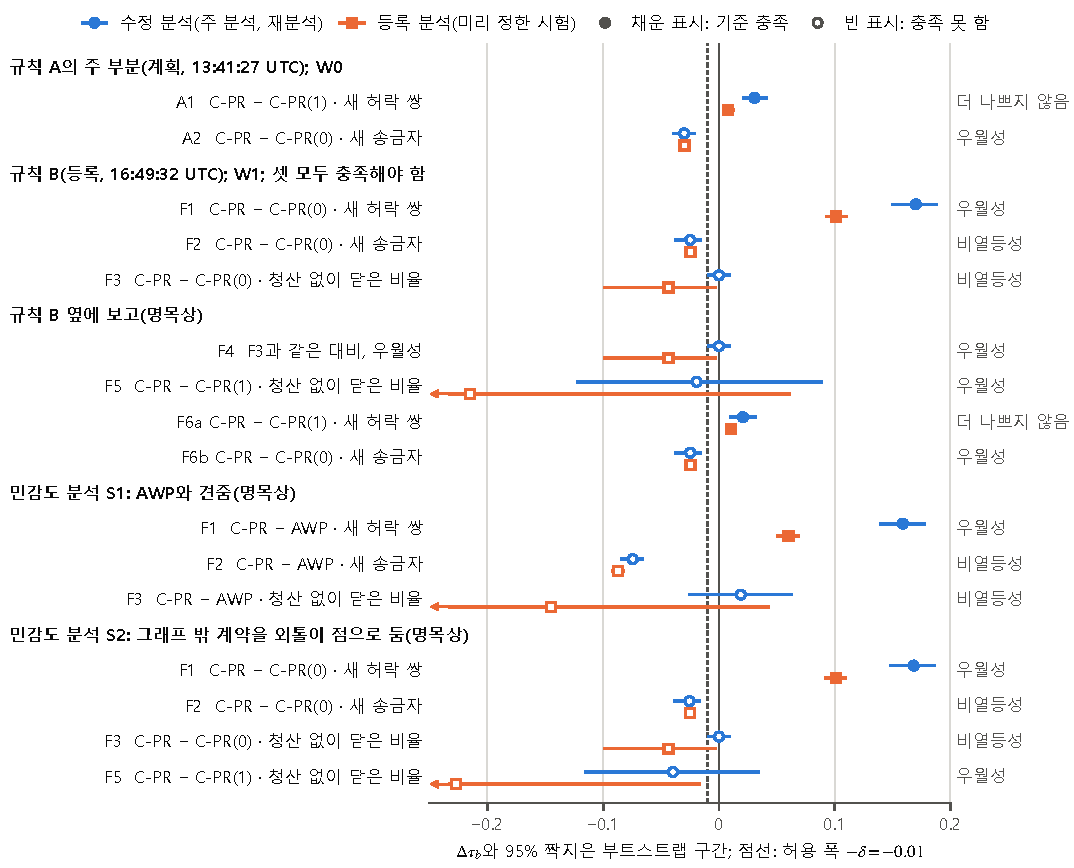
\includegraphics[width=\linewidth]{figures/fig_contrasts.pdf}
\caption{규칙 A와 B가 정한 대비, 규칙 B 옆에 보고하기로 등록한 결과, 그리고 등록한 민감도 분석 두 개. 95\% 짝지은 부트스트랩 구간이에요(다시 뽑기 400번, 시드 42). 동그라미는 수정 분석이에요. 주 분석이고, 달러 금액, 다섯 토큰, 동결 직전 12개월의 점수를 등록 결과를 안 뒤에 정해서 같은 규칙으로 다시 한 재분석이에요. 네모는 등록 분석, 곧 미리 정한 시험이에요. 채운 표시는 기준 충족, 빈 표시는 충족 못 함이에요. 점선은 허용 폭 $-\delta=-0.01$이고, 화살표는 그린 범위를 넘어가는 구간 끝이에요. 규칙을 판정하는 것은 A1--A2와 F1--F3뿐이고, 나머지 판정은 명목상이에요. S1의 F4는 그 F3과 같은 대비라 뺐어요. 값은 표~\ref{tab:contrasts}에 있어요.}
\label{fig:forest}
\end{figure}

\begin{puri}[그림~\ref{fig:forest}를 읽는 법]
한 줄이 대비 하나예요. 점은 $\Delta\tau$, 가로 선은 그 95\% 구간이에요. 세로 실선은 0, 점선은 허용 폭 −0.01이에요. 오른쪽 끝의 글자는 그 줄에 쓰는 기준(우월성, 비열등성, 더 나쁘지 않음)이에요. 예를 들어 F2 줄은 파란 선과 주황 선이 모두 점선의 왼쪽에 통째로 있어요. 두 분석 모두 C-PR이 송금 걷기보다 허용 폭 넘게 뒤졌다는 뜻이에요.
\end{puri}

\begin{table}[!ht]
\centering
\caption{동결 시점의 점수와 나중 라벨 사이의 켄달 $\tau_b$와 95\% 짝지은 부트스트랩 구간}
\label{tab:holdout}
\linespread{1}\selectfont\footnotesize
\setlength{\tabcolsep}{2.4pt}
\begin{tabular}{@{}L{3.5cm}C{2.0cm}C{2.0cm}C{2.0cm}C{2.0cm}C{2.0cm}@{}}
\toprule
\multicolumn{6}{@{}l}{\emph{(가) 수정 분석: 주 분석이며 미리 정한 규칙에 따른 재분석(달러 금액, 다섯 토큰, 12개월 점수 기간)}} \\
 & \multicolumn{2}{c}{W0 스펜더($n=7{,}914$)} & \multicolumn{2}{c}{W1 스펜더($n=7{,}960$)} & W1 트레이더($n=70$) \\
\cmidrule(lr){2-3}\cmidrule(lr){4-5}\cmidrule(l){6-6}
점수 & 새 허락 쌍 & 새 송금자 & 새 허락 쌍 & 새 송금자 & 청산 없이 닫은 비율 \\
\midrule
동결 시점의 받은 허락 수 & \tc{0.392}{[0.377, 0.406]} & \tc{0.284}{[0.267, 0.299]} & \tc{0.381}{[0.365, 0.396]} & \tc{0.269}{[0.250, 0.285]} & \tc{0.394}{[0.261, 0.524]} \\
동결 시점의 송금 입차수 & \tc{0.203}{[0.183, 0.224]} & \tc{0.447}{[0.435, 0.459]} & \tc{0.165}{[0.143, 0.186]} & \tc{0.439}{[0.426, 0.454]} & \tc{0.253}{[0.116, 0.363]} \\
EndorseRank & \tc{0.303}{[0.287, 0.319]} & \tc{0.272}{[0.257, 0.286]} & \tc{0.299}{[0.284, 0.314]} & \tc{0.259}{[0.243, 0.275]} & \tc{0.297}{[0.174, 0.418]} \\
AWP & \tc{0.196}{[0.178, 0.213]} & \tc{0.409}{[0.396, 0.421]} & \tc{0.157}{[0.137, 0.178]} & \tc{0.398}{[0.386, 0.412]} & \tc{0.263}{[0.140, 0.379]} \\
C-PR ($\lambda=1$), 허락 걷기 & \tc{0.298}{[0.282, 0.313]} & \tc{0.267}{[0.250, 0.282]} & \tc{0.295}{[0.280, 0.310]} & \tc{0.257}{[0.241, 0.274]} & \tc{0.302}{[0.177, 0.425]} \\
C-PR ($\lambda=0.75$) & \tc{0.327}{[0.311, 0.342]} & \tc{0.327}{[0.313, 0.339]} & \tc{0.316}{[0.298, 0.330]} & \tc{0.315}{[0.299, 0.329]} & \tc{0.284}{[0.160, 0.398]} \\
C-PR ($\lambda=0.5$), 주 설정 & \tc{0.329}{[0.312, 0.343]} & \tc{0.336}{[0.322, 0.348]} & \tc{0.316}{[0.300, 0.330]} & \tc{0.324}{[0.308, 0.337]} & \tc{0.282}{[0.162, 0.397]} \\
C-PR ($\lambda=0.25$) & \tc{0.329}{[0.312, 0.343]} & \tc{0.345}{[0.330, 0.357]} & \tc{0.315}{[0.299, 0.328]} & \tc{0.332}{[0.317, 0.346]} & \tc{0.282}{[0.162, 0.397]} \\
C-PR ($\lambda=0$), 송금 걷기 & \tc{0.178}{[0.160, 0.197]} & \tc{0.366}{[0.351, 0.378]} & \tc{0.146}{[0.126, 0.168]} & \tc{0.348}{[0.335, 0.363]} & \tc{0.282}{[0.162, 0.394]} \\
S-PR & \tc{0.190}{[0.171, 0.209]} & \tc{0.377}{[0.363, 0.389]} & \tc{0.162}{[0.140, 0.184]} & \tc{0.367}{[0.354, 0.381]} & \tc{0.300}{[0.175, 0.411]} \\
\bottomrule
\end{tabular}
\end{table}

\begin{table}[!ht]
\ContinuedFloat
\centering
\caption{(이어서) 등록 분석}
\linespread{1}\selectfont\footnotesize
\setlength{\tabcolsep}{2.4pt}
\begin{tabular}{@{}L{3.5cm}C{2.0cm}C{2.0cm}C{2.0cm}C{2.0cm}C{2.0cm}@{}}
\toprule
\multicolumn{6}{@{}l}{\emph{(나) 등록 분석: 미리 정한 시험(원래 단위, 모든 ERC-20 토큰)}} \\
 & \multicolumn{2}{c}{W0 스펜더($n=33{,}101$)} & \multicolumn{2}{c}{W1 스펜더($n=34{,}587$)} & W1 트레이더($n=70$) \\
\cmidrule(lr){2-3}\cmidrule(lr){4-5}\cmidrule(l){6-6}
점수 & 새 허락 쌍 & 새 송금자 & 새 허락 쌍 & 새 송금자 & 청산 없이 닫은 비율 \\
\midrule
동결 시점의 받은 허락 수 & \tc{0.252}{[0.244, 0.260]} & \tc{0.156}{[0.148, 0.166]} & \tc{0.262}{[0.255, 0.269]} & \tc{0.179}{[0.171, 0.186]} & \tc{0.394}{[0.261, 0.524]} \\
동결 시점의 송금 입차수 & \tc{0.148}{[0.138, 0.158]} & \tc{0.302}{[0.294, 0.310]} & \tc{0.145}{[0.135, 0.155]} & \tc{0.303}{[0.296, 0.309]} & \tc{0.331}{[0.209, 0.441]} \\
EndorseRank & \tc{0.241}{[0.234, 0.248]} & \tc{0.226}{[0.219, 0.234]} & \tc{0.233}{[0.226, 0.240]} & \tc{0.210}{[0.203, 0.217]} & \tc{0.306}{[0.176, 0.421]} \\
AWP & \tc{0.196}{[0.187, 0.206]} & \tc{0.340}{[0.333, 0.348]} & \tc{0.177}{[0.166, 0.187]} & \tc{0.322}{[0.316, 0.329]} & \tc{0.240}{[0.090, 0.362]} \\
C-PR ($\lambda=1$), 허락 걷기 & \tc{0.228}{[0.219, 0.236]} & \tc{0.122}{[0.113, 0.133]} & \tc{0.227}{[0.219, 0.234]} & \tc{0.133}{[0.125, 0.142]} & \tc{0.310}{[0.181, 0.432]} \\
C-PR ($\lambda=0.75$) & \tc{0.236}{[0.229, 0.243]} & \tc{0.217}{[0.209, 0.226]} & \tc{0.237}{[0.230, 0.244]} & \tc{0.228}{[0.220, 0.236]} & \tc{0.088}{[−0.110, 0.269]} \\
C-PR ($\lambda=0.5$), 주 설정 & \tc{0.236}{[0.229, 0.243]} & \tc{0.224}{[0.216, 0.234]} & \tc{0.237}{[0.230, 0.244]} & \tc{0.235}{[0.227, 0.243]} & \tc{0.095}{[−0.102, 0.274]} \\
C-PR ($\lambda=0.25$) & \tc{0.234}{[0.227, 0.241]} & \tc{0.230}{[0.222, 0.240]} & \tc{0.235}{[0.228, 0.242]} & \tc{0.240}{[0.232, 0.247]} & \tc{0.101}{[−0.096, 0.280]} \\
C-PR ($\lambda=0$), 송금 걷기 & \tc{0.142}{[0.133, 0.151]} & \tc{0.254}{[0.246, 0.262]} & \tc{0.136}{[0.125, 0.145]} & \tc{0.260}{[0.252, 0.266]} & \tc{0.138}{[−0.048, 0.310]} \\
S-PR & \tc{0.177}{[0.167, 0.186]} & \tc{0.245}{[0.236, 0.253]} & \tc{0.169}{[0.159, 0.178]} & \tc{0.251}{[0.244, 0.258]} & \tc{0.312}{[0.183, 0.422]} \\
\bottomrule
\end{tabular}

\vspace{4pt}
\parbox{\linewidth}{\footnotesize W0은 2026년 3월 31일에 점수를 동결하고 2026년 4–6월에 라벨을 세요. W1은 2026년 6월 30일에 동결하고 2026년 7–9월에 세요. 수정 분석은 모든 점수를 그 동결 직전 12개월로, 등록 분석은 2023년 10월 1일부터 추출한 모든 사건으로 만들어요. 스펜더는 동결 시점에 양수의 마지막 허락을 가진 계약이에요. 트레이더는 계약 코드를 가지고, 동결일 그래프의 점이며, 라벨 기간에 포지션을 셋 이상 닫은 GMX V2 계정이에요. 수정 분석에서 W0 스펜더 가운데 1{,}732개가 새 허락 쌍을, 1{,}422개가 새 송금자를 얻었고, W1에서는 1{,}495개와 1{,}371개가 얻었어요. 등록 분석에서는 3{,}403개, 3{,}042개, 2{,}850개, 2{,}812개예요. W1 트레이더 70개 가운데 9개가 청산을 한 번 이상 겪었어요. 받은 허락 수, 송금 입차수, EndorseRank, AWP의 행은 기준 점수이고, 그 비교는 짝 연구~\cite{kwon2026companion}가 모두 보고해요. 구간은 코호트의 계약을 다시 뽑은 짝지은 다시 뽑기 400번(시드 42)에서 왔어요.}
\end{table}

규칙 A에 없던 비교 하나는 반대쪽을 가리켰어요. 규칙 B를 쓸 때 있던 유일한 분석인 등록 분석에서, C-PR은 새 허락 쌍을 송금 걷기 혼자보다 훨씬 잘 줄 세웠어요(0.236 대 0.142, +0.094 [0.085, 0.103]). 이 대비는 라벨을 안 뒤에 살펴본 것이라 가설로 다뤘어요. 그래서 이 연구가 아직 추출하지 않은 창에서 그것을 시험하도록 규칙 B를 썼어요. 수정 점수로는 +0.151 [0.130, 0.170]이에요.

\begin{table}[!p]
\centering
\caption{두 분석의 짝지은 대비: 미리 정한 규칙, 등록한 보고와 민감도 분석, 라벨을 안 뒤에 계산한 대비}
\label{tab:contrasts}
\linespread{1}\selectfont\scriptsize
\setlength{\tabcolsep}{2.2pt}
\begin{tabular}{@{}L{4.45cm}L{1.9cm}C{2.75cm}C{1.45cm}C{2.75cm}C{1.45cm}@{}}
\toprule
 & & \multicolumn{2}{c}{수정 분석(재분석)} & \multicolumn{2}{c}{등록 분석(시험)} \\
\cmidrule(lr){3-4}\cmidrule(l){5-6}
대비($a-b$)와 라벨 & 기준 & $\Delta\tau$ [95\% 구간] & 판정 & $\Delta\tau$ [95\% 구간] & 판정 \\
\midrule
\multicolumn{6}{@{}l}{\emph{규칙 A: 이 연구가 로그를 하나도 추출하기 전에 계획(43d8045)에 정함; W0 스펜더}} \\
A1: C-PR − C-PR ($\lambda=1$), 새 허락 쌍 & 더 나쁘지 않음 & +0.031 [0.021, 0.042] & 성립 & +0.008 [0.003, 0.013] & 성립 \\
A2: C-PR − C-PR ($\lambda=0$), 새 송금자 & 우월성 & −0.030 [−0.040, −0.020] & 실패 & −0.030 [−0.034, −0.026] & 실패 \\
규칙 A의 주 부분(A1과 A2) & & & \textbf{충족 못 함} & & \textbf{충족 못 함} \\
규칙 A의 부 부분(같은 기간) & & & \textbf{충족 못 함} & & \textbf{충족 못 함} \\
\midrule
\multicolumn{6}{@{}l}{\emph{규칙 B: 이 연구가 W1 로그를 추출하기 전에 등록(0d3a057); F1, F2, F3 모두 필요; 허용 폭 $\delta=0.01$}} \\
F1: C-PR − C-PR ($\lambda=0$), 새 허락 쌍 & 우월성 & +0.170 [0.149, 0.189] & 성립 & +0.101 [0.092, 0.111] & 성립 \\
F2: C-PR − C-PR ($\lambda=0$), 새 송금자 & 비열등성 & −0.025 [−0.038, −0.015] & 실패 & −0.025 [−0.029, −0.021] & 실패 \\
F3: C-PR − C-PR ($\lambda=0$), 청산 없는 비율 & 비열등성 & +0.000 [−0.010, 0.010] & 실패 & −0.044 [−0.100, −0.002] & 실패 \\
규칙 B(F1, F2, F3) & & & \textbf{충족 못 함} & & \textbf{충족 못 함} \\
\midrule
\multicolumn{6}{@{}l}{\emph{판정 옆에 정해진 순서로 보고하기로 등록함(명목상)}} \\
F4: F3과 같은 대비 & 우월성 & +0.000 [−0.010, 0.010] & 실패 & −0.044 [−0.100, −0.002] & 실패 \\
F5: C-PR − C-PR ($\lambda=1$), 청산 없는 비율 & 우월성 & −0.019 [−0.123, 0.089] & 실패 & −0.215 [−0.472, 0.062] & 실패 \\
F6a: C-PR − C-PR ($\lambda=1$), 새 허락 쌍 & 더 나쁘지 않음 & +0.021 [0.009, 0.032] & 성립 & +0.010 [0.005, 0.014] & 성립 \\
F6b: C-PR − C-PR ($\lambda=0$), 새 송금자 & 우월성 & −0.025 [−0.038, −0.015] & 실패 & −0.025 [−0.029, −0.021] & 실패 \\
\midrule
\multicolumn{6}{@{}l}{\emph{등록한 민감도 분석 S1: AWP를 비교 대상으로(명목상)}} \\
F1: C-PR − AWP, 새 허락 쌍 & 우월성 & +0.159 [0.139, 0.178] & 성립 & +0.060 [0.050, 0.070] & 성립 \\
F2: C-PR − AWP, 새 송금자 & 비열등성 & −0.075 [−0.085, −0.065] & 실패 & −0.087 [−0.093, −0.082] & 실패 \\
F3: C-PR − AWP, 청산 없는 비율 & 비열등성 & +0.019 [−0.026, 0.064] & 실패 & −0.145 [−0.348, 0.043] & 실패 \\
\midrule
\multicolumn{6}{@{}l}{\emph{등록한 민감도 분석 S2: 그래프 밖 계약을 외톨이 점으로 둠(명목상)}} \\
F1: C-PR − C-PR ($\lambda=0$), 새 허락 쌍 & 우월성 & +0.168 [0.147, 0.187] & 성립 & +0.101 [0.091, 0.111] & 성립 \\
F2: C-PR − C-PR ($\lambda=0$), 새 송금자 & 비열등성 & −0.025 [−0.039, −0.016] & 실패 & −0.025 [−0.029, −0.022] & 실패 \\
F3: C-PR − C-PR ($\lambda=0$), 청산 없는 비율 & 비열등성 & +0.000 [−0.010, 0.010] & 실패 & −0.044 [−0.100, −0.002] & 실패 \\
F5: C-PR − C-PR ($\lambda=1$), 청산 없는 비율 & 우월성 & −0.040 [−0.116, 0.035] & 실패 & −0.227 [−0.426, −0.016] & 실패 \\
S1의 판정(F1, F2, F3) & & & \textbf{충족 못 함} & & \textbf{충족 못 함} \\
S2의 판정(F1, F2, F3) & & & \textbf{충족 못 함} & & \textbf{충족 못 함} \\
\midrule
\multicolumn{6}{@{}l}{\emph{그 창의 라벨을 안 뒤에 계산함; 규칙 없음}} \\
W0: C-PR − C-PR ($\lambda=0$), 새 허락 쌍 & --- & +0.151 [0.130, 0.170] & & +0.094 [0.085, 0.103] & \\
W0: S-PR − C-PR ($\lambda=1$), 새 허락 쌍 & --- & −0.108 [−0.128, −0.088] & & −0.051 [−0.060, −0.043] & \\
W0: S-PR − C-PR ($\lambda=0$), 새 송금자 & --- & +0.011 [0.004, 0.018] & & −0.009 [−0.012, −0.006] & \\
W0: C-PR − AWP, 새 송금자 & --- & −0.073 [−0.083, −0.063] & & −0.116 [−0.122, −0.109] & \\
W0: C-PR ($\lambda=1$) − 받은 허락 수, 새 허락 쌍 & --- & −0.094 [−0.104, −0.083] & & −0.025 [−0.030, −0.019] & \\
W0: EndorseRank − 받은 허락 수, 새 허락 쌍 & --- & −0.090 [−0.100, −0.079] & & −0.011 [−0.016, −0.006] & \\
W0: AWP − 송금 입차수, 새 송금자 & --- & −0.038 [−0.043, −0.032] & & +0.038 [0.035, 0.042] & \\
W1: EndorseRank − 받은 허락 수, 새 허락 쌍 & --- & −0.082 [−0.090, −0.073] & & −0.029 [−0.032, −0.025] & \\
W1: AWP − 송금 입차수, 새 송금자 & --- & −0.041 [−0.047, −0.034] & & +0.020 [0.016, 0.023] & \\
W1: C-PR − EndorseRank, 새 허락 쌍 & --- & +0.017 [0.006, 0.029] & & +0.004 [−0.001, 0.008] & \\
\bottomrule
\end{tabular}

\vspace{4pt}
\parbox{\linewidth}{\footnotesize $\Delta\tau=\tau_a-\tau_b$를 같은 다시 뽑기에서 구해요. $\lambda$ 없이 쓴 C-PR은 주 설정 $\lambda=0.5$예요. 청산 없는 비율은 W1 트레이더의 청산 없이 닫은 비율이에요. 우월성은 구간이 0보다 위일 때, 비열등성은 아래 끝이 $-\delta=-0.01$보다 위일 때, “더 나쁘지 않음”은 구간이 0을 포함하거나 0보다 위일 때 성립해요. 수정 분석 열은 주 분석이에요. 계획과 등록의 규칙과 기준을, 등록 결과를 안 뒤에 정한 점수(달러 금액, 다섯 토큰, 동결 직전 12개월의 점수)에 적용했으므로, 그 판정은 어느 것도 등록한 결과가 아니에요. 등록 분석 열이 계획과 등록이 정한 시험이에요. 명목상의 판정은 보정하지 않은 95\% 구간을 써요. 정해진 순서는 보고하는 순서였을 뿐, 관문 순서가 아니었어요. 받은 허락 수, 송금 입차수, EndorseRank, AWP의 행은 기준 대비이고 \cite{kwon2026companion}이 모두 보고해요. 구간은 짝지은 다시 뽑기 400번(시드 42)에서 왔어요.}
\end{table}

\subsection{W1: 규칙 B는 충족 못 함}

\paragraph{수정 분석.}
\begin{itemize}
\item \textbf{F1은 성립해요.} 나중에 허락 쌍을 얻는 스펜더를 C-PR은 $\tau=0.316$ [0.300, 0.330]으로, 송금 걷기는 0.146 [0.126, 0.168]으로 줄 세워요. 차이는 +0.170 [0.149, 0.189]예요. W0의 이득이, 규칙을 정한 뒤 이 연구가 추출한 창에서 다시 나타난 거예요.
\item \textbf{F2는 실패해요.} 새 송금자에서 C-PR은 0.324 [0.308, 0.337], 송금 걷기는 0.348 [0.335, 0.363]이에요. 차이 −0.025 [−0.038, −0.015]의 구간 전체가 허용 폭 −0.01 너머에 있어요. 그래서 자료는, 나중의 송금자를 줄 세우는 데서 C-PR이 송금 걷기에 등록이 허용한 폭보다 더 크게 뒤진다는 것을 보여 줘요.
\item \textbf{F3은 아슬아슬하게 실패해요.} 트레이더의 청산 없이 닫은 비율에서 C-PR은 0.282 [0.162, 0.397], 송금 걷기도 0.282 [0.162, 0.394]예요. 그 차이 +0.000 [−0.010, 0.010]의 구간은 아래 끝이 −0.01보다 아주 조금 낮아요.
\end{itemize}
규칙은 셋 모두를 요구하므로 충족되지 않았어요. 그래서 이 원고는 C-PR이 송금 걷기보다 낫다고 주장하지 않아요.

\begin{puri}[구간이 {[−0.010, 0.010]}인데 왜 실패인가요?]
표의 수는 소수 셋째 자리로 반올림한 값이에요. 실제 아래 끝은 −0.01보다 아주 조금 낮아서, 아래 끝이 $-\delta$보다 위에 있어야 한다는 비열등성 기준을 넘지 못했어요. 이 실패가 두 걷기의 차이가 아니라 다시 뽑기에 달려 있다는 것은 \ref{sec:precision}절에서 다뤄요.
\end{puri}

\paragraph{등록 분석.}
등록이 정한 시험인 등록 분석도 같은 판정에 이르러요(표~\ref{tab:contrasts}).
\begin{itemize}
\item F1은 성립해요(+0.101 [0.092, 0.111]; 0.237 대 0.136).
\item F2는 구간 전체가 허용 폭 너머라 실패해요(−0.025 [−0.029, −0.021]; 0.235 대 0.260).
\item F3도 실패해요. C-PR은 0.095 [−0.102, 0.274], 송금 걷기는 0.138 [−0.048, 0.310]이고, 차이는 −0.044 [−0.100, −0.002]예요. 등록한 시드에서는 구간이 0 아래에 있지만, 다른 시드에서는 0에 닿기도 해요(부록~\ref{app:explore}).
\end{itemize}
등록이 F3에 대해 미리 걱정한 약점이 이 분석에서 실제로 일어났어요. 두 걷기 계수의 구간이 모두 0을 포함하는데, 같은 라벨에서 허락 걷기는 0.310 [0.181, 0.432], 받은 허락 수는 0.394 [0.261, 0.524]에 이르렀어요.

그래서 두 분석은 F3에서 성격이 달라요.
\begin{itemize}
\item 등록 분석에서는 원래 단위 금액의 송금 걷기와 C-PR이 모두 트레이더를 약하게 줄 세웠고, C-PR의 계수가 더 낮았어요.
\item 수정 분석에서는 표~\ref{tab:holdout}의 모든 점수가 0보다 위인 구간으로 트레이더를 줄 세웠고, C-PR은 송금 걷기와 같았으며 정밀도 때문에만 실패했어요.
\end{itemize}
두 분석 모두에서 이 라벨의 가장 높은 계수는 받은 허락 수의 것이에요. 그리고 라벨을 안 뒤에 수정 점수 파일로 계산한 대비에서, C-PR은 트레이더를 받은 허락 수만큼 잘 줄 세우지 못해요(−0.112 [−0.194, −0.026]).

\subsection{판정 옆에 보고하는 결과}

이 판정들은 명목상이에요. 각각 보정하지 않은 95\% 구간을 쓰고, 어느 것도 다른 것의 결과에 조건을 걸지 않았어요. 두 분석 모두에서 이래요.
\begin{itemize}
\item \textbf{F4는 실패해요.} 트레이더 라벨에서 C-PR이 송금 걷기보다 앞서지 않아요.
\item \textbf{F5는 실패해요.} 그 라벨에서 C-PR과 허락 걷기를 가를 수 없어요(수정 −0.019 [−0.123, 0.089], 등록 −0.215 [−0.472, 0.062]).
\item \textbf{F6은 W0처럼 실패해요.} 규칙 A의 주 부분을 W1에서 다시 한 것이에요. C-PR은 새 허락 쌍에서 허락 걷기보다 나쁘지 않지만(+0.021 [0.009, 0.032], +0.010 [0.005, 0.014]), 새 송금자에서는 송금 걷기보다 못해요.
\end{itemize}

민감도 분석은 어느 분석에서도 판정을 바꾸지 않아요.
\begin{itemize}
\item \textbf{S1(AWP를 비교 대상으로).} F1은 성립해요(수정 +0.159 [0.139, 0.178], 등록 +0.060 [0.050, 0.070]). F2는 구간 전체가 허용 폭보다 한참 아래라 실패해요. AWP는 새 송금자를 수정 분석에서 0.398 [0.386, 0.412], 등록 분석에서 0.322 [0.316, 0.329]로 줄 세우고, C-PR의 모자람은 −0.075 [−0.085, −0.065]와 −0.087 [−0.093, −0.082]예요. 그러니 발표된 송금 기반 방법과 견주면, C-PR은 나중 허락에서의 이득을 얻는 대신 나중 유입을 줄 세우는 힘을 눈에 띄게 내줘요. S1의 F3도 실패해요(+0.019 [−0.026, 0.064], −0.145 [−0.348, 0.043]). 트레이더 70개에서 수정 구간의 폭은 0.090이라, 0.026만큼 손해일 가능성도 남겨 두지만 손해를 보여 주지는 않아요.
\item \textbf{S2(빠진 계약을 외톨이 점으로).} 판정은 하나도 바뀌지 않고, F1–F3의 점 추정값은 많아야 0.002 움직여요. F5는 더 움직여요. 외톨이 점 규칙이 허락 그래프 밖의 트레이더를 0점에서 “들어오는 화살표가 없는 점”의 점수로 올려서, 허락 걷기의 동점 구조를 바꾸기 때문이에요. 수정 분석에서 허락 걷기의 트레이더 라벨 계수는 0.302에서 0.322로 오르고 F5는 여전히 판가름 나지 않아요(−0.040 [−0.116, 0.035]). 등록 분석에서는 F5가 판가름 난 모자람이 돼요(−0.227 [−0.426, −0.016]).
\end{itemize}

\subsection{무게 훑기}
\label{sec:sweep}

그림~\ref{fig:sweep}은 각 라벨을 $\lambda$에 따라 그려요.
\begin{itemize}
\item \textbf{새 허락 쌍.} 큰 걸음은 아래 끝에서 와요. 허락 층을 켜면 C-PR이 수정 W1에서 0.146에서 0.315로, 등록 W1에서 0.136에서 0.235로 올라요. 안쪽 값들끼리는 0.003보다 적게 달라요.
\item \textbf{새 송금자.} 안쪽 곡선은 $\lambda$가 커질수록 천천히 내려가요(수정 W1에서 0.332, 0.324, 0.315, 등록 W1에서 0.240, 0.235, 0.228). 안쪽 값은 모두 송금 걷기보다 낮아요. 위 끝에서는 허락 걷기가 새 송금자에서 뚝 떨어져요(0.257과 0.133). $\lambda=1$에서는 허락 화살표가 없는 계약의 송금 행이 사라지기 때문이에요.
\item \textbf{트레이더 라벨.} 수정 곡선은 안쪽에서 0.282–0.284로 평평해요. 송금 걷기(0.282)와 같고, 허락 걷기(0.302)보다 조금 낮아요. 등록 곡선은 0.088과 0.101 사이에 머물러서, 0.138인 송금 걷기와 0.310인 허락 걷기보다 낮아요.
\end{itemize}
그러니 송금 걷기보다 나은 F1의 이득은 허락 층을 \emph{켜는 것}의 성질이지, $\lambda=0.5$라는 값의 성질이 아니에요. 그리고 어떤 안쪽 값도 송금 걷기가 나중 송금자를 줄 세우는 힘을 되찾지 못해요. 부록~\ref{app:explore}가 $\lambda$를 0에서 0.25로, 0.25에서 0.75로, 0.75에서 1로 옮길 때의 짝지은 걸음과, 이 값들 사이의 순위 일치를 보여 줘요.

\begin{figure}[!ht]
\centering
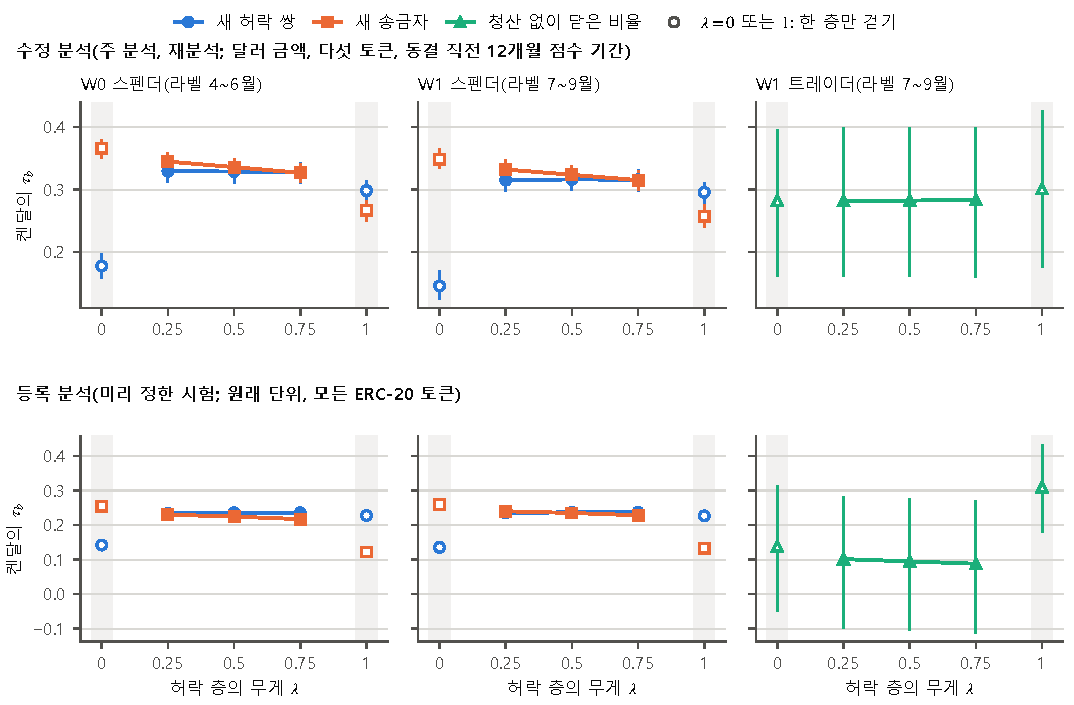
\includegraphics[width=\linewidth]{figures/fig_lambda_sweep.pdf}
\caption{허락 층의 무게 $\lambda$에 따른, C-PR과 각 나중 라벨 사이의 켄달 $\tau_b$와 95\% 짝지은 부트스트랩 구간. 선으로 이은 채운 표시는 미리 정한 격자 $\lambda\in\{0.25,0.5,0.75\}$예요. 회색 띠 안의 빈 표시는 $\lambda=0$과 $\lambda=1$, 곧 송금 걷기와 허락 걷기예요. 선이 잇지 않는 별개의 연산자예요. 위 줄은 수정 분석(주 분석, 재분석), 아래 줄은 등록 분석(미리 정한 시험)이에요. 줄마다 세로축을 같이 써요. 값은 표~\ref{tab:holdout}에 있어요.}
\label{fig:sweep}
\end{figure}

\subsection{씨앗 재시작}

S-PR은 새 송금자에서는 송금 걷기에 가깝고, 새 허락 쌍에서는 허락 걷기보다 한참 아래에 머물러요.
\begin{itemize}
\item W0에서 새 허락 쌍의 S-PR − 허락 걷기는 수정 분석에서 −0.108 [−0.128, −0.088], 등록 분석에서 −0.051 [−0.060, −0.043]이에요.
\item 새 송금자의 S-PR − 송금 걷기는 +0.011 [0.004, 0.018]과 −0.009 [−0.012, −0.006]이에요.
\item 다시 출발은 새 허락 쌍의 계수를 송금 걷기에서 허락 걷기 쪽으로 일부만 끌어올려요. 수정 W0에서 0.190이고 송금 걷기는 0.178, 허락 걷기는 0.298이에요. 등록 W0에서는 0.177 대 0.142와 0.228이에요. 송금 걷기와의 짝지은 대비는 계산하지 않았어요.
\end{itemize}
$d=0.85$이면 몫의 15\%와 매달린 점의 몫만 다시 출발 벡터를 지나요. 그래서 허락 화살표는 걷기를 실어 나를 때, 곧 허락 걷기에서는 온전히, C-PR에서는 섞여서 쓰일 때 나중 허락에 도움이 되고, 다시 출발할 곳만 정할 때는 거의 도움이 되지 않아요.

나중 송금자에서는 순서가 뒤집혀요. 라벨을 안 뒤에 수정 점수 파일로 계산한 대비에서, C-PR은 두 창 모두에서 새 허락 쌍은 S-PR보다 더 잘 줄 세우지만(+0.139 [0.121, 0.156], +0.154 [0.134, 0.174]), 새 송금자는 S-PR만큼 잘 줄 세우지 못해요(−0.041 [−0.049, −0.032], −0.044 [−0.052, −0.037]).

\subsection{걷기 대 수}

어떤 걷기도 새 허락 쌍을 원시 받은 허락 수만큼 잘 줄 세우지 못했어요. 두 분석 모두 점 추정값으로 그랬고, 계산한 짝지은 대비마다 그랬어요.
\begin{itemize}
\item \textbf{W0.} 허락 걷기는 받은 허락 수에 수정 분석에서 −0.094 [−0.104, −0.083], 등록 분석에서 −0.025 [−0.030, −0.019]만큼 모자라요. 엔도스랭크는 −0.090 [−0.100, −0.079]와 −0.011 [−0.016, −0.006]만큼 모자라요.
\item \textbf{W1.} 엔도스랭크는 −0.082 [−0.090, −0.073]과 −0.029 [−0.032, −0.025]만큼 모자라요. 허락 걷기의 점 추정값도 받은 허락 수보다 낮아요(0.295 대 0.381, 0.227 대 0.262). 짝지은 대비는 계산하지 않았어요.
\item \textbf{라벨을 안 뒤에 수정 점수 파일로 계산한 짝지은 대비.} C-PR은 두 창 모두에서 받은 허락 수에 모자라요(−0.063 [−0.076, −0.052], −0.065 [−0.077, −0.054]). AWP의 활동 재시작을 쓴 엔도스랭크도 그래요(−0.060 [−0.070, −0.052], −0.046 [−0.055, −0.038]). 등록 분석에서 C-PR의 새 허락 쌍 점 추정값은 두 창 모두 받은 허락 수보다 아래예요(표~\ref{tab:holdout}). 짝지은 대비는 계산하지 않았어요.
\end{itemize}

새 송금자에서도 수정 분석에서는 수가 앞서요. C-PR은 두 창 모두에서 새 송금자를 송금 입차수만큼 잘 줄 세우지 못하고(−0.111 [−0.121, −0.100], −0.115 [−0.128, −0.105]), AWP도 그래요(W0 −0.038 [−0.043, −0.032], W1 −0.041 [−0.047, −0.034]). 반면 등록 분석에서는 AWP가 송금 입차수보다 더 잘 줄 세워요(+0.038 [0.035, 0.042], +0.020 [0.016, 0.023]). 균등 재시작과 상한 없는 금액을 쓰는 C-PR의 송금 걷기는, 모든 경우에 송금 입차수보다 점 추정값이 낮아요.

기준 비교는 짝 연구가 모두 보고해요~\cite{kwon2026companion}. 여기서 되풀이하는 까닭은, 이 비교가 이 원고의 어떤 걷기든 주장할 수 있는 범위를 묶기 때문이에요. 허락 쪽은 명제~\ref{prop:closed}가 설명해요. 대부분의 스펜더에서 걷기는 무게를 다시 단 주인 수이고, 이 도착 라벨에서는 다시 단 무게가 도움이 되지 않았어요. 차수 결과는 선호적 연결~\cite{barabasi1999scaling,newman2001clustering}, 그리고 링크 예측에서 차수 기준선이 강하다는 것~\cite{libennowell2007link,lin2022tracking}과 맞아요.

\subsection{라벨을 본 뒤, 기준 걷기와 견주기}
\label{sec:reference}

규칙 A와 B는 C-PR을 자기 층과 견줘요. 결합만을 바꾸는 대비는 그것뿐이기 때문이에요. 짝 연구의 기준 걷기와의 대비는 라벨을 안 뒤에 수정 점수 파일로, 규칙과 같은 다시 뽑기를 써서 계산했어요. 이 대비들이 C-PR의 자리를 더 밝혀 줘요. 어느 것도 규칙에 들어가지 않고, 표~\ref{tab:contrasts}의 두 행 말고는 등록 분석에 짝이 없어요.
\begin{itemize}
\item \textbf{엔도스랭크와.} 각 스펜더 라벨과 각 창에서 C-PR이 앞서요. 새 허락 쌍에서 +0.026 [0.016, 0.037]과 +0.017 [0.006, 0.029], 새 송금자에서 +0.064 [0.052, 0.075]와 +0.064 [0.051, 0.076]이에요.
\item \textbf{활동 재시작 엔도스랭크와.} 새 허락 쌍에서 W0에서는 같고(−0.003 [−0.014, 0.008]), W1에서는 못해요(−0.019 [−0.029, −0.008]).
\item \textbf{AWP와.} 새 허락 쌍에서 C-PR이 앞서는 것(W0 +0.133 [0.114, 0.153], W1 +0.159 [0.139, 0.178], S1의 F1)은 대부분 송금 화살표가 없어서 AWP가 0점을 주는 스펜더에서 와요. 동결 전에 들어온 송금이 있는 스펜더(W0 6,489개, W1 6,567개)만 보면, 새 허락 쌍에서 C-PR과 AWP는 W0에서 같고(+0.008 [−0.002, 0.020]) W1에서 C-PR이 0.022 [0.011, 0.033] 앞서요. 반면 새 송금자에서는 AWP가 0.036 [0.026, 0.044]와 0.037 [0.028, 0.046]만큼 더 잘 줄 세워요. 모든 스펜더에서도 그랬어요(W0에서 0.073 [0.063, 0.083], W1에서 0.075 [0.065, 0.085]).
\end{itemize}
그러니 기간 밖에서 허락 층이 송금 걷기에 더해 주는 것은 주로, 송금 걷기가 동점으로 남겨 두는 계약들 사이의 순서예요. 나머지 계약들 사이에서는 W1에서 나중 허락에 작은 앞섬이 있을 뿐이에요. 나중 송금자에서는 C-PR이 모든 부분 집합과 창에서 AWP보다 뒤져요.

\subsection{정밀도와 허용 폭}
\label{sec:precision}

허용 폭은 스펜더 대비의 정밀도에서 나왔고, 그대로 트레이더 대비에 적용했어요.
\begin{itemize}
\item \textbf{스펜더에서는 지킬 수 있는 폭이었어요.} F2의 구간 폭은 수정 분석에서 0.023, 등록 분석에서 0.008이에요. F2가 실패한 것은 구간이 넓어서가 아니라, 구간 전체가 허용 폭 너머에 있었기 때문이에요.
\item \textbf{트레이더에서는 계약 70개로 겨우 닿는 폭이었어요.} F3의 구간 폭은 수정 분석에서 0.020, 등록 분석에서 0.098이에요. 두 계수가 같으면, 수정 F3은 구간이 약 $2\delta$보다 좁을 때만 성립할 수 있어요. 등록한 시드에서 반폭은 0.01004이고, 다른 부트스트랩 시드 50개에서 아래 끝은 −0.0146에서 −0.0098 사이이며, 한 시드에서는 아래 끝이 −0.01보다 위로 올라와 기준을 통과해요(부록~\ref{app:explore}).
\end{itemize}
그래서 수정 F3의 실패는 두 걷기의 차이가 아니라 다시 뽑기에 달려 있어요. 반면 등록 분석의 반폭(0.049)은 허용 폭의 약 5배이고, 등록 F3의 위 끝은 시드 50개 가운데 11개에서 0 이상에 닿아요. 스펜더 구간의 끝은 시드에 따라 거의 움직이지 않고(표준편차 0.0002–0.0015), 규칙 B는 F2 때문에 두 분석의 모든 시드에서 실패해요.

스펜더 쪽 라벨은 듬성듬성해요. 수정 W1 스펜더 7,960개 가운데 1,495개만 새 허락 쌍을, 1,371개만 새 송금자를 얻었어요(등록 분석에서는 34,587개 가운데 2,850개와 2,812개). 그래서 스펜더 계수는 저마다 그 부분 집합들의 순서에 크게 기대요.

\begin{puri}[허용 폭을 지키려면 구간이 얼마나 좁아야 하나요?]
두 계수가 같으면 차이의 점 추정값이 0이에요. 비열등성은 아래 끝이 −0.01보다 위에 있어야 하므로, 구간의 아래쪽 반이 0.01보다 짧아야 해요. 곧 구간 전체의 폭이 약 $2\delta$보다 좁아야 해요. 수정 F3의 폭은 0.020이라 딱 그 경계에 걸렸고, 시드에 따라 통과하기도 해요. 등록 F3은 반폭이 0.049라, 계수가 같았더라도 통과할 수 없는 폭이었어요.
\end{puri}

%======================================================================
\section{허락 층의 시빌 노출}
\label{sec:sybil}

\begin{yoji}
허락 하나에는 수수료만 들고 토큰이 묶이지 않아요. 균등 재시작으로 허락 층을 걷는 점수에서 닫힌 농장은 자기 인구 몫의 몇 배를 모아요. 수정 분석의 엔도스랭크 그래프에서는 주소 26개짜리 별 모양이면 목표를 코호트 점수의 상위 10\%로 올려요(등록 그래프에서는 13개). 결합한다고 이 빈틈이 닫히지는 않는다는 것도 논리로 보여요. 이 모형은 W1 라벨을 안 뒤에 계산했고 어느 규칙에도 들어가지 않아요.
\end{yoji}

앞의 결과는 정직한 자료에 관한 것이에요. 평판 층은 속이는 데 드는 비용으로도 판단해야 해요. 이 절은 Gy\"{o}ngyi와 Garcia-Molina의 농장 결과~\cite{gyongyi2005alliances}를, 균등 재시작을 쓰는 엔도스랭크의 허락 걷기에 맞춰 수치로 재요. 그래프는 수정 분석의 2026년 6월 30일 동결 그래프(점 2,513,982개, 화살표 3,808,949개)이고, 등록 분석의 그래프를 견줘 보여요. 닫힌 농장의 한계(식~\eqref{eq:farm})는 이 층을 균등 재시작으로 걷는 걷기라면 무엇에나, $\lambda=1$의 C-PR에도 성립해요. 하지만 아래의 별 모양 수는 코호트의 엔도스랭크 점수에 견줘 읽어요. 이 모형은 W1 라벨을 안 뒤에 계산했고 어느 규칙에도 들어가지 않아요.

\subsection{화살표 하나의 비용}

스펜더를 허락해도 아무것도 맡겨 두지 않아요. 토큰이 묶이지 않고, 허락하는 주소는 그 토큰을 하나도 갖지 않아도 돼요. 상한이 있는 무게에서는 몇백 달러짜리 허락이 무제한 허락과 거의 같은 무게를 가져요. 그리고 행을 정규화하면, 나가는 화살표가 하나뿐인 점은 금액이 얼마든 그 화살표가 행 전체를 가져요. 그래서 공격자의 두 주소 사이의 화살표는 아무것도 위험에 내놓지 않고, 수수료만 들어요.

수정 그래프는 동결 직전 12개월 동안 정한 허락만 담아요. 그래서 허락은 정한 지 1년이 지나면 엔도스랭크에서도, C-PR의 허락 층에서도 빠져요. 따라서 농장은 적어도 1년에 한 번은 허락을 다시 내야 해요. 닫힌 농장 안에서는 엔도스랭크의 나이 할인이 상관없어요. 농장 주소의 행은 모두 농장 안에 머무는 화살표들끼리 정규화되기 때문이에요. 이런 기간을 $q$번 거치는 동안 닫힌 농장의 비용은 다음과 같아요.
\begin{equation}
C=q\,\bigl(|E_{\mathcal S}|\,c_{\text{gas}}+c_{\text{rev}}\bigr).
\label{eq:cost}
\end{equation}
$c_{\text{gas}}$는 허락 하나의 수수료이고, $c_{\text{rev}}$는 기간마다 허락을 거두거나 들키지 않으려고 드는 비용이에요. $c_{\text{gas}}$는 재지 않았어요. 값이 얼마든 비용은 화살표 수와 기간 수에 따라 선형으로 늘어요. 그래프를 널리 거래되는 다섯 토큰으로 한정해도 이 비용은 오르지 않아요. 그 가운데 하나를 허락하는 것이 다른 토큰을 허락하는 것보다 비싸지 않기 때문이에요. 다섯 토큰으로 한정해서 없어지는 것은, 실제로 움직인 적 없는 주인의 이름으로 토큰 계약이 써 넣은 로그예요.

\subsection{닫힌 농장이 모으는 것}

농장 $\mathcal S$의 모든 점이 나가는 화살표를 가지되 그 화살표가 모두 농장 안을 가리키고, 정직한 주인은 아무도 농장 주소를 허락하지 않는다고 해요. 매달린 점들이 가진 정상 몫을 $r_D$라고 써요. 매달린 점은 모두 정직한 점이에요. 균등한 $\boldsymbol\pi$로 식~\eqref{eq:pr}을 $\mathcal S$에 걸쳐 더하면 다음이 나와요.
\begin{equation}
\sum_{i\in\mathcal S} r_i=\frac{|\mathcal S|}{|V|}\cdot\frac{1-d+d\,r_D}{1-d}\le\frac{|\mathcal S|}{(1-d)|V|+d|\mathcal S|}.
\label{eq:farm}
\end{equation}
부등식은 $r_D\le 1-\sum_{i\in\mathcal S}r_i$를 써서 얻어요. 둘째 인수는 농장이 자기 인구 몫의 몇 배를 차지하는지를 나타내요. 매달린 점이 있으면 그 몫이 다시 나눠져 농장에도 닿으므로, 이 배수는 늘 1보다 커요.
\begin{itemize}
\item 수정 그래프에서 $d=0.75$, $0.85$, $0.95$일 때 $r_D=0.365$, $0.394$, $0.419$예요. 그래서 닫힌 농장은 자기 인구 몫의 2.10배, 3.23배, 8.96배를 차지해요.
\item 주소 20개가 다음 주소를 하나씩 허락하는 고리를 그래프에 넣어 보면, $d=0.85$에서 자기 몫의 3.23배를 차지해요.
\item 등록 그래프에서는 배수가 2.01, 2.96, 6.62예요.
\end{itemize}

\begin{puri}[왜 인구 몫보다 더 많이 모이나요?]
걷는 사람이 매달린 점에 도착하면 그 몫은 모든 점에 고르게 다시 나눠져요. 농장 주소도 그 일부를 받아요. 그런데 닫힌 농장에서는 화살표가 모두 농장 안을 가리키므로, 받은 몫이 순간 이동(확률 $1-d$)으로만 빠져나가요. 그래서 몫이 농장 안에 쌓이고, 매달린 점의 몫 $r_D$가 클수록, 그리고 $d$가 1에 가까울수록 더 많이 쌓여요.
\end{puri}

\subsection{몫을 한곳에 모으기}

식~\eqref{eq:farm}는 농장 전체의 몫을 묶을 뿐이고, 공격자는 그 몫을 한 점에 모을 수 있어요. 별 모양에서는 농장 주소 $f$개가 모두 목표 $t$를 허락하고, $t$도 그 주소들을 하나하나 허락해요. 순간 이동과 매달린 행에서 각 점이 받는 몫을 $c=(1-d+d\,r_D)/|V|$로 두면, 균형 식에서 다음이 나와요.
\begin{equation}
r_t=\frac{c\,(1+d\,f)}{1-d^{2}}.
\label{eq:star}
\end{equation}
\begin{itemize}
\item 수정 그래프에서 $c=1.93\times10^{-7}$이에요. 들어오는 화살표가 없는 모든 점의 공통 점수예요.
\item $f=10$이면 주소 11개와 기간마다 허락 20개로, 목표는 별을 넣은 그래프에서 $6.60\times10^{-6}$을 받아요. 식~\eqref{eq:star}의 값이에요. 코호트 점수의 중앙값($5.82\times10^{-7}$)보다 위이고, 90번째 백분위($1.56\times10^{-5}$)의 5분의 2쯤이에요.
\item 농장 주소를 하나 더할 때마다 기간마다 허락 2개를 더 내고 $d\,c/(1-d^2)$를 더 얻어요.
\end{itemize}
식~\eqref{eq:star}을 $f$에 대해 풀면 각 순위에 드는 비용이 나와요.
\begin{itemize}
\item 중앙값에는 별이 아예 필요 없어요. 서로를 허락하는 주소 둘만으로 이미 $c/(1-d)$에 이르러요.
\item 90번째 백분위에는 농장 주소 26개가 들어요.
\item 99번째 백분위($1.35\times10^{-3}$)에는 약 2,292개가 들어요.
\item 코호트 계약 가운데 가장 높은 점수(0.0278)에는 약 47,073개가 들어요. 이 수는 그렇게 큰 농장이 $|V|$를 키워 $c$를 낮추는 효과를 무시한 값이에요.
\item 등록 그래프에서는 이 수가 13, 1,253, 약 1,080,271이에요.
\end{itemize}
그래서 농장은 기간마다 허락 52개로 코호트 점수의 상위 10분의 1에 들어가요(등록 그래프에서는 26개). 그 수수료는 재지 않았어요. 반면 맨 꼭대기에는 천 배가 넘게 큰 농장이 필요해요. 앞선 계약들이 정상 몫의 큰 부분을 쥐고 있기 때문이에요.

\begin{puri}[별 모양 농장의 셈을 따라가 보면]
별 모양에서 목표 $t$는 농장 주소 $f$개에게서 허락을 받고, 그 주소들에게 다시 허락을 줘요. 걷는 사람은 $t$와 농장 주소 사이를 오가므로, 순간 이동으로 들어온 몫이 $t$에 거듭 돌아와 쌓여요. 식~\eqref{eq:star}에서 $f$가 하나 늘면 $t$의 점수는 일정한 양만큼 늘어요. 그래서 수정 그래프에서는 상위 10\%에 몇십 개의 주소로 닿지만, 이미 큰 몫을 쥔 맨 위 계약을 넘으려면 주소가 몇만 개나 필요해요.
\end{puri}

\subsection{결합 걷기에서도 같은 논리}

$\lambda>0$인 C-PR에서는 식~\eqref{eq:alpha}의 다시 정규화 때문에, 나가는 화살표가 모두 허락인 점은 그 화살표를 무게 1로 따라가요. 그래서 서로만 허락하고 송금을 하지 않는 농장은, 허락 걷기에서와 똑같이 C-PR에서도 닫혀 있어요. 식~\eqref{eq:farm}는 C-PR의 매달린 몫으로 그대로 들어맞아요. 다만 저자들은 그 몫을 계산하지도, C-PR의 그래프에서 농장을 돌려 보지도 않았어요. 그래서 위의 배수를 C-PR에 대해 주장하지 않아요. 이 논리는 결합이 빈틈을 닫지 못한다는 것만 보여 줘요.

상한을 둔 C-PR의 층에서, 정직한 주인에게서 산 허락 하나가 몫을 크게 옮기는 것은 그 허락이 그 주인의 다른 허락에 견줘 클 때뿐이에요. 그리고 상한만큼의 허락이면 스펜더는 그 주인에게서 적어도 $U$달러를 꺼낼 수 있어요. 반면 엔도스랭크의 상한 있는 층에서는, 새로 낸 몇백 달러짜리 허락 하나가 중앙값 주인의 행에서 68.3\%를 차지해요. 대부분 주인의 마지막 허락이 오래됐거나 작기 때문이에요.

\subsection{처방, 시험하지 않음}

Cheng과 Friedman이 찾은 비대칭이 해결책을 가리켜요~\cite{cheng2005sybilproof}. 트러스트랭크처럼~\cite{gyongyi2004trustrank} 뛰기와 매달린 점의 몫을 검증한 씨앗 집합으로만 보내면, 씨앗 밖의 농장은 정직한 주인에게서 오는 화살표로만 몫을 얻어요. 그리고 그 화살표는 돈을 주고 사야 해요. 저자들은 씨앗으로 제한한 재시작을 평가하지 않았어요. S-PR은 그런 처방이 아니에요. S-PR의 씨앗은 농장이 부풀릴 수 있는 허락 점수이기 때문이에요. 휴먼 패스포트~\cite{humanpassportnddocs} 같은 자격 증명 관문은 다른 질문, 곧 한 주소가 서로 다른 한 사람의 것인지를 다뤄요. 이 질문은 계약에는 바로 맞는 짝이 없고, 그런 관문에는 나름의 약점이 있어요~\cite{bordeianu2026sybil}. 이 분석은 모형에 바탕을 두고, 관측한 그래프에서 풀이 프로그램으로 점검했어요. 체인 위에서 실제로 공격해 보지는 않았어요.

%======================================================================
\section{타당성을 위협하는 것}
\label{sec:threats}

\begin{yoji}
스펜더 라벨은 같은 종류의 화살표가 새로 생기는 것이라 지금의 수를 따라가는 점수에 유리해요. 수정 분석(달러 금액, 다섯 토큰, 12개월 점수 기간)은 등록 결과를 안 뒤에 정했고, 등록은 제3자의 시간 도장이 없으며, 트레이더는 70개뿐이에요. 증거는 한 롤업, 한 걸음 에고 네트워크, 고정된 전체 무게에서 나왔어요.
\end{yoji}

\subsection{구성 타당도}

\begin{itemize}
\item 스펜더 라벨은 층을 이루는 것과 같은 종류의 화살표가 새로 생기는 것이에요. 그래서 미래의 연결을 재고, 지금의 수를 따라가는 점수에 유리해요. 둘 다 신용, 안전, 손실의 결과가 아니에요.
\item 트레이더 라벨은 이 자료에서 부도에 가장 가까운 결과예요. 하지만 한 거래소에서의 강제 청산은 대출의 부도가 아니고, W1 트레이더 70개 가운데 9개만 청산을 겪었어요.
\item 허락 화살표는 기준 시점까지의 마지막 허락이지, 지금 유효한 허락이 아니에요(\ref{sec:model}절). 수정 분석에서는 12개월 점수 기간 전에 정한 허락은 아무리 오래 유효해도 세지 않아요. 동결 블록의 계약 상태에서 허락을 읽으면, 새 쌍으로 센 것 가운데 몇 개가 다시 낸 옛 관계였는지 가릴 수 있어요.
\item 층의 무게가 중요해요. 계획대로의 원래 금액 층에서는 무제한 허락과 소수 자릿수가 큰 토큰이 행을 차지했고, 수정 분석의 달러 금액과 상한이 그것을 막아요.
\item 두 분석은 규칙 A와 B에서 같은 판정에 이르렀어요. 하지만 둘은 무게, 토큰, 점수 기간이 한꺼번에 달라서, 어느 하나를 훑어본 것이 아니에요. 엔도스랭크와 AWP의 상한 있는 무게를 쓰는 층처럼 다른 결합은 이 원고에서 평가하지 않았어요.
\end{itemize}

\subsection{내적 타당도}

\begin{itemize}
\item 규칙 A는 이 연구가 로그를 하나도 추출하기 전에 정했어요. 규칙 B의 가설은 W0의 탐색적 대비에서, 그 허용 폭은 W0의 구간에서 나왔어요.
\item 등록은 저자들 자신의 저장소에 있는 커밋이지, 독립 등록처의 항목이 아니에요. 등록이 W1 추출보다 먼저였다는 것은 제3자의 시간 도장이 아니라 커밋 시각과 작업 시각에 기대요(\ref{sec:gate}절).
\item 달러 금액, 다섯 토큰, 12개월 점수 기간을 쓰는 수정 분석은 모든 등록 결과를 안 뒤에 정했어요. 그래서 그 선택이 한쪽 결과에 유리했을 수 있어요. 두 사실이 그 위험을 줄이지만 없애지는 못해요. 기울기와 상한은 W0 동결까지 12개월의 사건 분위수에서 나와서 라벨 기간의 사건이 들어가지 않아요. 그리고 수정 분석은 규칙 A와 B에서 등록 분석과 같은 판정에 이르렀어요.
\item 수정 분석을 먼저 보고하는 것도 결과를 본 뒤의 선택이에요. 등록 분석은 규칙을 정할 때 시험하려던 분석으로서, 결과의 모든 표와 그림에 남아 있어요.
\item 빠진 계약을 0점으로 두는 규칙은 처리 과정의 선택이에요. S2는 이 규칙이 등록 분석의 F5를 동점 구조를 통해 바꾸지만, 판정의 어느 부분도 바꾸지 않는다는 것을 보여 줘요.
\end{itemize}

\subsection{통계적 결론 타당도}

\begin{itemize}
\item 규칙에 묶인 구간은 계획에서 정한 대로 짝지은 다시 뽑기 400번에서 나와요. 그 몬테카를로 오차는 판정을 가른 거리에 견주면 작아요. 예외는 수정 F3이에요. 그 아래 끝은 허용 폭에 걸려 있고, 다른 시드 50개 가운데 하나에서는 아래 끝이 −0.01보다 위로 올라와 기준을 통과해요(부록~\ref{app:explore}). 규칙 B의 판정은 그 시드에 기대지 않아요. F2가 모든 시드에서 실패하기 때문이에요.
\item 판정은 세 조건의 교집합이라 다중 비교 보정이 필요 없어요. 하지만 판정 옆에 보고한 많은 대비는 명목상이라, 한 묶음의 시험으로 읽으면 안 돼요.
\item 계약을 다시 뽑는 부트스트랩은 스펜더들을 서로 독립으로 다뤄요. 그런데 새 주인 하나가 여러 스펜더를 허락할 수 있어요.
\item 트레이더 코호트는 작아요. 스펜더에서 가져온 허용 폭은 수정 분석에서는 트레이더가 겨우 닿는 경계에, 등록 분석에서는 닿지 않는 곳에 있었어요(\ref{sec:precision}절).
\end{itemize}

\subsection{외적 타당도}

증거는 한 롤업, 주인 셋 이상에게 허락을 받은 그 롤업의 계약, 동결 직전 1년으로 만든 점수(등록 분석에서는 2023년 10월부터의 모든 사건), 석 달짜리 라벨 기간 두 개에서 나왔어요. 각 그래프는 코호트의 한 걸음 에고 네트워크라서, 나가는 무게와 걷는 길은 체인 전체가 아니라 그 에고 네트워크의 것이에요. 보증이 한 걸음보다 멀리 퍼지는 더 깊은 표본에서는 다르게 움직일 수 있어요. 시험한 것은 균등 순간 이동을 쓰는 고정된 전체 무게뿐이에요. 점마다 다른 무게나 학습한 무게, 정상 벡터의 혼합, 층 사이에 점의 복사본을 두는 방식, 층마다 다른 감쇠 계수는 열린 문제로 남아 있어요.

%======================================================================
\section{대출과 마진 프로토콜에 주는 시사점}
\label{sec:implications}

\begin{yoji}
가장 싼 점수인 원시 차수는 자기 구성개념에서는 이기기 어려웠어요. 두 신호를 하나의 정상 분포로 섞기보다 나란히 보고할 수 있어요. 균등 재시작으로 허락을 걷는 점수는 농장으로 부풀릴 수 있고, 허락은 사건 로그가 아니라 계약 상태에서 읽어야 해요.
\end{yoji}

온체인 관계로 상대나 연동을 거르는 프로토콜~\cite{bartoletti2021lending,perez2021liquidations}은 이 결과에서 실용적인 점 네 가지를 얻을 수 있어요.
\begin{enumerate}
\item \textbf{가장 싼 점수인 원시 차수는 자기 구성개념에서는 이기기 어려웠어요.} 계약을 허락한 서로 다른 주인 수를 세는 것이, 결합 걷기를 포함한 이 연구의 모든 걷기보다 그 계약의 나중 허락을 잘 예상했어요. 수정 분석에서는 서로 다른 송금자 수를 세는 것이 AWP와 결합 걷기보다 나중 송금자를 잘 예상했어요. 풀이 프로그램도, 지켜야 할 다시 출발 벡터도 필요 없어요. 다만 원시 차수가 더 속이기 어려운 것은 아니에요. 새 주소 $N$개의 허락은 허락 수수료 $N$번으로 그 수를 $N$만큼 올려요.
\item \textbf{섞어서 얻은 이득에는 손실도 따랐어요.} 허락 층을 송금 걷기에 섞으면 순위는 주로 허락 층을 켜는 것으로 움직였어요. 그리고 나중 허락에서의 이득에는 등록한 허용 폭보다 큰 나중 송금에서의 손실이 따라왔어요. 두 신호를 모두 원하는 프로토콜은 두 원시 차수를, 또는 AWP와 받은 허락 수를, 하나의 정상 분포로 접지 말고 나란히 보고할 수 있어요.
\item \textbf{농장으로 부풀릴 수 있어요.} 균등 재시작으로 허락 화살표를 걷는 점수는 무엇이든, 토큰 없이 허락 수수료만 드는 닫힌 농장으로 부풀릴 수 있어요. 그 수수료는 재지 않았어요. 수정 그래프에서는 농장 주소 스물몇 개면 코호트 엔도스랭크 점수의 상위 10분의 1에 닿아요(26개, 등록 그래프에서는 13개). 그래프가 지난 1년의 허락만 담으므로, 농장은 1년에 한 번 허락을 다시 내서 화살표를 유지해요. 이론이 가리키는 처방은 다시 출발을 검증한 씨앗으로 제한하는 것이지만, 시험하지 않았어요.
\item \textbf{허락 로그는 허락의 상태가 아니에요.} 허락에 따라 움직이는 프로토콜은 사건 기간에서 허락을 다시 짜 맞추지 말고, 결정하는 블록의 계약 상태에서 허락을 읽어야 해요.
\end{enumerate}

%======================================================================
\section{결론}
\label{sec:conclusion}

\begin{yoji}
결합 걷기는 나중 허락에서는 송금 걷기를 앞섰지만 나중 송금에서는 송금 걷기보다 뒤져서(규칙 B에서는 허용 폭보다 더), 두 규칙을 모두 충족하지 못했어요. 수정 분석과 등록 분석의 판정이 같았어요. 라벨을 안 뒤에 계산한 대비 여럿에서, 결합 걷기는 원시 차수와 기준 걷기만큼 잘 줄 세우지 못했어요.
\end{yoji}

허락과 송금은 같은 계약을 두 가지로 읽어 줘요. 이 표본에서 모든 점에서 두 층을 섞는 걷기는 나중의 허락을 어느 한 층보다 잘 줄 세웠어요. 허락 걷기보다는 조금 나았을 뿐이에요. 하지만 나중의 송금자는 송금 걷기보다 못하게 줄 세웠어요. 그래서 두 라벨 모두에서 두 층을 이기지는 못했어요.

주 분석은 다섯 토큰의 달러 금액과 동결 직전 1년의 점수 기간을 써요. 이 달러 금액, 다섯 토큰, 1년 점수 기간은 계획대로 한 분석의 결과를 안 뒤에 정했으므로, 주 분석은 같은 규칙에 따른 재분석이에요. 이 분석에서 C-PR은 첫 창에서 나중 허락을 허락 걷기보다 나쁘지 않게 줄 세웠지만, 나중 송금자에서 송금 걷기를 이기지 못했어요. 그래서 이 연구가 로그를 하나도 추출하기 전에 계획에서 정한 규칙은 충족되지 않았어요.

이 연구가 추출하기 전에 등록한 창에서, C-PR은 나중 허락에서 송금 걷기보다 나은 점을 되풀이했어요(+0.170 [0.149, 0.189]). 하지만 나중 송금자는 등록한 허용 폭보다 더 못하게 줄 세웠고(−0.025 [−0.038, −0.015]), AWP와 견주면 그보다 더 못했어요. 계약 트레이더의 청산 없는 거래에서는 송금 걷기와 같았지만(+0.000 [−0.010, 0.010]), 허용 폭 안에 머물 만큼 정밀하지 못했어요. 두 규칙이 시험하려던 분석, 곧 원래 단위로 미리 정한 분석도 같은 판정에 이르렀어요. 등록한 세 기준에서 +0.101 [0.092, 0.111], −0.025 [−0.029, −0.021], −0.044 [−0.100, −0.002]였어요.

허락에서의 이득은 허락 층을 켜자마자 나타나고, 안쪽 무게들 사이에서는 거의 바뀌지 않아요. 송금 걷기에 허락 점수로 씨앗을 주면 그 이득의 일부만 되찾았어요. 라벨을 안 뒤에 계산한 대비에서, C-PR은 두 스펜더 라벨 모두에서 엔도스랭크보다 더 잘 줄 세웠고, 나중 허락에서 AWP를 앞선 것은 대부분 AWP가 0점을 주는 계약에서 왔어요. 그 대비 가운데 여럿은 C-PR에게 불리했어요.
\begin{itemize}
\item 나중 허락은 두 창 모두에서 허락한 주인 수(원시 차수)만큼, 두 번째 창에서는 활동 재시작 엔도스랭크만큼 잘 줄 세우지 못했어요.
\item 나중 송금자는 두 창 모두에서 송금자 수(원시 차수)와 AWP만큼 잘 줄 세우지 못했어요.
\item 트레이더의 청산 없이 닫은 비율은 받은 허락 수만큼 잘 줄 세우지 못했어요.
\end{itemize}
균등 재시작에서는 1년에 몇십 개의 허락으로 허락 층을 부풀릴 수 있고, 결합은 이 노출을 없애지 못해요.

앞으로의 연구는 다음을 미리 정하고, 제3자의 시간 도장으로 묶어 두고, 아직 추출하지 않은 자료에서 시험해야 해요. 두 층에 같은 꼴의 무게를 다는 결합(예를 들어 두 층 모두 상한 있는 무게), 여러 걸음의 퍼뜨림이 나타날 만큼 깊은 표본, 허용 폭을 지킬 만큼 큰 트레이더 코호트, 그리고 명시적인 공격 아래에서 씨앗으로 제한한 재시작이에요.

%======================================================================
\appendix
\section{탐색적 점검}
\label{app:explore}

\begin{yoji}
판정 대비를(S2 제외) 발표된 점수 파일에서 다시 계산하면 발표된 값과 정확히 같아요. 다른 시드 50개에서도 규칙 B는 늘 실패해요. 수정 F3만 한 시드에서 아래 끝이 −0.01보다 위로 올라와 기준을 통과해요. 안쪽 $\lambda$ 값들의 순위는 거의 같고, 두 끝점은 다른 연산자예요.
\end{yoji}

아래 점검은 모두 두 분석의 모든 결과를 안 뒤에 보조 자료의 스크립트로 돌렸어요. 스크립트는 발표된 계약별 점수 파일과 요약을 읽을 뿐, 그래프를 만들지 않아요. 어느 점검도 규칙에 들어가지 않아요. 표~\ref{tab:explore}이 결과를 보여 줘요.

\paragraph{다시 계산.}
스크립트는 점수 파일에서 A1, A2, F1–F6, S1을 두 분석 모두 다시 계산해요. 처리 과정의 다시 뽑기와 SciPy의 $\tau_b$를 쓰고, 다시 계산한 값은 모두 발표된 값과 같아요. S2는 다시 계산할 수 없어요. 한 층 걷기의 외톨이 점 점수가 점수 파일에 없기 때문이에요.

\paragraph{시드에 따른 퍼짐.}
다시 뽑기 400번짜리 시드를 50개 더 써도, A1, A2, F1, F2의 판정은 두 분석 모두 바뀌지 않고, 규칙 B는 모든 시드에서 실패해요(표~\ref{tab:explore}(a)). 스펜더 대비에서 구간 끝의 표준편차는 0.0002–0.0015예요. 트레이더 대비 F3에서는 더 많이 움직여요.
\begin{itemize}
\item 수정 F3의 아래 끝은 −0.0146에서 −0.0098 사이이고, 50개 시드 가운데 하나에서는 아래 끝이 −0.01보다 위로 올라와 기준을 통과해요. 그러니 등록한 시드에서의 아슬아슬한 실패는 다시 뽑기에 기댄 것이지, 계수가 같은 두 걷기의 차이에 기댄 것이 아니에요.
\item 등록 분석에서 F3은 아래 끝이 −0.11 근처에 머물러 모든 시드에서 실패해요. 하지만 위 끝은 50개 가운데 11개 시드에서 0 이상에 닿아요. 그래서 “C-PR이 트레이더를 송금 걷기보다 못하게 줄 세웠다”는 해석은 시드에 기대요. 규칙의 실패는 그렇지 않아요.
\item 두 분석 모두 트레이더 다시 뽑기 20,000개 가운데 하나는 라벨이 모두 같은 값이라 건너뛰었어요.
\end{itemize}

\paragraph{무게의 걸음.}
\begin{itemize}
\item 허락 층을 켜면($\lambda$를 0에서 0.25로) 새 허락 쌍의 $\tau_b$가 0.092–0.169만큼 오르고, 새 송금자의 $\tau_b$는 0.016–0.024만큼 내려가요. 두 창과 두 분석 모두에서 구간이 0을 벗어나요(표~\ref{tab:explore}(b)).
\item $\lambda=0.25$와 0.75 사이에서는 새 허락 쌍의 변화가 어느 쪽으로든 많아야 0.002이고, 새 송금자에서는 −0.012에서 −0.018 사이예요.
\item 송금 층을 끄면($\lambda$를 0.75에서 1로) 두 스펜더 라벨이 모두 내려가요. 새 허락 쌍에서 0.008–0.029만큼, 새 송금자에서 0.058–0.095만큼이에요.
\item 트레이더 라벨에서는 등록 분석의 0에서 0.25로 가는 걸음만 구간이 0을 벗어나요(−0.037 [−0.085, −0.001]). 등록 분석의 0.75에서 1로 가는 걸음은 +0.222 [−0.062, 0.487], 수정 분석의 같은 걸음은 +0.018 [−0.091, 0.125]예요.
\end{itemize}

\paragraph{순위 일치.}
$\lambda=0.25$와 $\lambda=0.75$의 C-PR 순위는 두 분석의 모든 코호트에서 $\tau_b$ 0.869에서 0.889 사이로 일치하고, 구간의 폭은 0.009를 넘지 않아요. 반면 각 끝점은 가장 가까운 안쪽 값과 0.557에서 0.624($\lambda=0$과 0.25), 0.596에서 0.660($\lambda=0.75$와 1) 사이로 일치해요(표~\ref{tab:explore}(c)). 안쪽이 라벨에서 평평한 까닭은 안쪽 무게들 사이에서 순위 자체가 거의 바뀌지 않기 때문이고, 두 끝점은 서로 다른 연산자예요.

\begin{table}[!p]
\centering
\caption{탐색적 점검. 두 분석의 결과를 모두 안 뒤에 계산했어요}
\label{tab:explore}
\linespread{1}\selectfont\scriptsize
\setlength{\tabcolsep}{2.4pt}
\begin{tabular}{@{}L{3.0cm}L{2.4cm}C{4.9cm}C{4.9cm}@{}}
\toprule
 & & 수정 분석 & 등록 분석 \\
\midrule
\multicolumn{4}{@{}l}{\emph{(a) 다른 부트스트랩 시드 50개(각 다시 뽑기 400번)에서의 판정 대비: 구간 끝의 평균(표준편차) [범위]; 판정이 시드 42와 다른 시드 수}} \\
A1, W0, 새 허락 쌍 & 위 끝 & \tc{0.0415 (0.0006) [0.0400, 0.0431];}{50개 중 0개} & \tc{0.0132 (0.0004) [0.0124, 0.0142];}{50개 중 0개} \\
A2, W0, 새 송금자 & 아래 끝 & \tc{−0.0399 (0.0006) [−0.0411, −0.0388];}{50개 중 0개} & \tc{−0.0336 (0.0002) [−0.0342, −0.0329];}{50개 중 0개} \\
F1, W1, 새 허락 쌍 & 아래 끝 & \tc{0.1507 (0.0015) [0.1479, 0.1531];}{50개 중 0개} & \tc{0.0926 (0.0006) [0.0905, 0.0939];}{50개 중 0개} \\
F2, W1, 새 송금자 & 아래 끝 & \tc{−0.0352 (0.0008) [−0.0376, −0.0339];}{50개 중 0개} & \tc{−0.0281 (0.0003) [−0.0287, −0.0275];}{50개 중 0개} \\
F3, W1, 청산 없이 닫은 비율 & 아래 끝 & \tc{−0.0121 (0.0011) [−0.0146, −0.0098];}{50개 중 1개} & \tc{−0.1064 (0.0044) [−0.1173, −0.0969];}{50개 중 0개} \\
\midrule
\multicolumn{4}{@{}l}{\emph{(b) 무게의 걸음: 높은 $\lambda$의 C-PR $\tau_b$에서 낮은 $\lambda$의 값을 뺀 짝지은 차이, 다시 뽑기 400번, 시드 42}} \\
W0 스펜더, 새 허락 쌍 & $0\to0.25$ & +0.151 [0.132, 0.170] & +0.092 [0.083, 0.101] \\
 & $0.25\to0.75$ & −0.002 [−0.005, 0.001] & +0.002 [0.000, 0.003] \\
 & $0.75\to1$ & −0.029 [−0.040, −0.018] & −0.008 [−0.013, −0.003] \\
W0 스펜더, 새 송금자 & $0\to0.25$ & −0.021 [−0.030, −0.012] & −0.024 [−0.027, −0.020] \\
 & $0.25\to0.75$ & −0.018 [−0.021, −0.015] & −0.013 [−0.015, −0.012] \\
 & $0.75\to1$ & −0.060 [−0.071, −0.048] & −0.095 [−0.102, −0.087] \\
W1 스펜더, 새 허락 쌍 & $0\to0.25$ & +0.169 [0.149, 0.187] & +0.099 [0.090, 0.109] \\
 & $0.25\to0.75$ & +0.001 [−0.002, 0.004] & +0.002 [0.001, 0.003] \\
 & $0.75\to1$ & −0.020 [−0.031, −0.009] & −0.010 [−0.014, −0.006] \\
W1 스펜더, 새 송금자 & $0\to0.25$ & −0.016 [−0.029, −0.007] & −0.020 [−0.023, −0.016] \\
 & $0.25\to0.75$ & −0.017 [−0.020, −0.014] & −0.012 [−0.013, −0.010] \\
 & $0.75\to1$ & −0.058 [−0.069, −0.045] & −0.095 [−0.102, −0.088] \\
W1 트레이더, 청산 없이 닫은 비율 & $0\to0.25$ & +0.000 [−0.007, 0.008] & −0.037 [−0.085, −0.001] \\
 & $0.25\to0.75$ & +0.002 [−0.010, 0.014] & −0.013 [−0.036, 0.002] \\
 & $0.75\to1$ & +0.018 [−0.091, 0.125] & +0.222 [−0.062, 0.487] \\
\midrule
\multicolumn{4}{@{}l}{\emph{(c) 순위 일치: 두 $\lambda$ 값의 C-PR 점수 사이의 $\tau_b$, 코호트 전체, 다시 뽑기 400번, 시드 42}} \\
매칭 코호트, 기간 끝 & $\lambda=0$과 $0.25$ & 0.587 [0.569, 0.602] & 0.624 [0.616, 0.632] \\
 & $\lambda=0.25$와 $0.75$ & 0.879 [0.875, 0.884] & 0.869 [0.867, 0.871] \\
 & $\lambda=0.75$와 $1$ & 0.596 [0.585, 0.610] & 0.618 [0.612, 0.624] \\
W0 스펜더 & $\lambda=0$과 $0.25$ & 0.557 [0.542, 0.572] & 0.598 [0.592, 0.605] \\
 & $\lambda=0.25$와 $0.75$ & 0.889 [0.886, 0.893] & 0.884 [0.882, 0.886] \\
 & $\lambda=0.75$와 $1$ & 0.659 [0.648, 0.670] & 0.658 [0.652, 0.663] \\
W1 스펜더 & $\lambda=0$과 $0.25$ & 0.558 [0.543, 0.573] & 0.594 [0.586, 0.600] \\
 & $\lambda=0.25$와 $0.75$ & 0.882 [0.879, 0.886] & 0.884 [0.882, 0.886] \\
 & $\lambda=0.75$와 $1$ & 0.622 [0.612, 0.634] & 0.660 [0.655, 0.665] \\
\bottomrule
\end{tabular}

\vspace{4pt}
\parbox{\linewidth}{\footnotesize 처리 과정의 계약별 점수 파일로, 두 분석의 결과를 모두 안 뒤에 계산했어요. 어느 행도 규칙에 들어가지 않아요. 스크립트는 먼저 표~\ref{tab:contrasts}의 판정 대비를 S2만 빼고 모두 다시 계산해서, 발표된 값을 정확히 재현해요. (a)에서 A1 행은 “더 나쁘지 않음”을 판정하는 위 끝을, 나머지 행은 아래 끝을 보여 줘요.}
\end{table}

%======================================================================
\section*{투고 서류에 들어가는 것}
\addcontentsline{toc}{section}{투고 서류에 들어가는 것}

\begin{yoji}
IEEE Access 양식의 나머지 부분이에요. 핵심어, 서지 정보, 감사의 말, 저자 기여, 이해 충돌, 자료 공개, 저자 소개가 있어요. 영문 원고에서는 핵심어와 서지 정보가 첫머리에, 나머지는 부록 A 뒤에 있어요.
\end{yoji}

\subsection*{핵심어}
블록체인, 탈중앙 금융, 다층 네트워크, 부정적 결과, 페이지랭크, 사전 등록, 평판 시스템, 스마트 계약, 시빌 공격, 토큰 허락.

\subsection*{서지 정보}
양식 머리의 출판 날짜와 DOI 칸에는 양식의 자리 표시가 들어 있어요. 날짜 칸은 xxxx 00, 0000이고, DOI 칸은 \path{10.1109/ACCESS.2024.0429000}이에요. 교신 저자는 Taehong Kwon(thkwon@enu-tech.co.kr)이에요. 이 연구는 외부 연구비를 받지 않았어요.

\subsection*{감사의 말}
저자들은 1저자의 박사 연구를 지원한 남아프리카 대학교(University of South Africa) 컴퓨팅 학부에 감사해요. 이 연구는 그 박사 연구의 일부예요. 사건 로그는 Google BigQuery에 있는 공개 아비트럼 원 자료에서 가져왔어요. 이 연구의 BigQuery 작업 56개에는 모두 합쳐 USD 42.24가 청구됐어요. 이 원고를 준비하면서 저자들은 글과 분석 스크립트의 언어 다듬기, 구성 고치기, 점검을 돕는 데 Claude(Anthropic)를 썼어요. 이 도구를 쓴 뒤 저자들은 내용을 검토하고 필요한 만큼 고쳤으며, 발표되는 글의 내용에 모든 책임을 져요.

\subsection*{저자 기여}
\begin{itemize}
\item Taehong Kwon: 연구 구상, 방법론, 소프트웨어, 자료 관리, 형식 분석, 초고 쓰기.
\item Ernest Mnkandla: 지도, 검토와 편집.
\item Donatien Koulla Moulla: 지도, 검토와 편집.
\item David Sena Attipoe: 지도, 검토와 편집.
\end{itemize}

\subsection*{이해 충돌}
저자들은 이 글이 보고하는 연구에 영향을 준 것처럼 보일 수 있는 금전적 이해관계나 개인적 관계를 알지 못한다고 밝혀요.

\subsection*{자료 공개}
이 연구는 공개 블록체인 자료, 공개된 하루 토큰 가격, 공개된 Chainlink 피드 목록만 쓰고, 사람 참여자가 없어요.
\begin{itemize}
\item 코드, 설정, 계획, 등록, 개정 문서, 추출 매니페스트, 비용 장부, 계약별 점수 파일, 기계가 읽는 결과 요약과 그 SHA-256 체크섬은 공개 저장소 \url{https://github.com/abitocodes/phd_works}의 폴더 \path{1-Dissertation-Works/ERC20-Allowance-PageRank-Wallet-Reputation/experiments}에 있어요. 표~\ref{tab:ids}의 처음 일곱 커밋에서는 이 폴더의 이름이 \path{ERC20-Allowance-PageRank-Contract-Reputation/experiments}예요.
\item 등록 결과는 \path{data/3-published-results-for-thesis/}에, 수정 결과는 그 아래 폴더 \path{revised-usd-12m/}에 있어요. 수정 결과는 \sha{950a7a4}에 커밋했고, 코드 리비전 \sha{0a94215}로 계산했어요.
\item 추출한 그래프 표는 저자들의 BigQuery 프로젝트에 보관해요. 커밋된 질의로 공개 로그 표에서 다시 만들 수 있어요.
\item 이 원고의 소스, 표와 그림 스크립트, 보조 자료(자료를 추출하고 모으는 질의, 탐색적 점검 스크립트와 그 출력)는 \url{https://github.com/abitocodes/phd-dissertation-draft-en}의 폴더 \path{manuscripts/B-ieee-access}에 있어요.
\end{itemize}
점수는 계약만 줄 세워요. 외부 소유 계정은 주인, 보낸 쪽, 받는 쪽으로 그래프에 들어가요. 블록체인 밖의 신원은 모으지도 잇지도 않았고, 원고는 모아 낸 결과만 보고해요.

\subsection*{저자 소개}
\begin{itemize}
\item \textbf{Taehong Kwon}: 남아프리카공화국 요하네스버그, 남아프리카 대학교 컴퓨팅 학부의 컴퓨터 과학 박사 후보생이에요. 관심 분야는 온체인 평판, 탈중앙 금융, 그래프 기반 순위 매기기예요.
\item \textbf{Ernest Mnkandla}: 같은 학부의 교수예요. 관심 분야는 소프트웨어 공학과 인공지능이에요.
\item \textbf{Donatien Koulla Moulla}: 같은 학부 CAIDS(Centre for Augmented Intelligence and Data Science) 소속이에요.
\item \textbf{David Sena Attipoe}: 같은 학부 CAIDS 소속이에요.
\end{itemize}


\bibliographystyle{IEEEtran}
\bibliography{../../overleaf-github/manuscripts/B-ieee-access/references}

\end{document}
